% =====================================================================
%  Master's thesis (English)  --  Hyun-Ju Lee
%  Generative discovery and first-principles validation of economical
%  high-entropy carbide electrocatalysts for CO2 electroreduction (CO2RR)
%
%  Compile:  xelatex main && xelatex main   (twice for ToC/refs)
%  Figures read from ../figures/ (CarbideMatterGen pipeline outputs).
% =====================================================================
\documentclass[11pt,a4paper]{report}

\usepackage[margin=2.5cm]{geometry}
\usepackage{graphicx}
\graphicspath{{../figures/}}
\usepackage{amsmath,amssymb}
\usepackage{booktabs}
% --- lightweight stand-ins for siunitx (avoids a package dependency) ---
\providecommand{\SI}[2]{#1\,#2}
\providecommand{\SIrange}[3]{#1--#2\,#3}
\providecommand{\si}[1]{#1}
\providecommand{\angstrom}{\mbox{\AA}}
\usepackage{xcolor}
\usepackage{caption}
\usepackage[hidelinks]{hyperref}
\usepackage{microtype}
\emergencystretch=3em
\usepackage{enumitem}
\usepackage{tikz}
\usetikzlibrary{arrows.meta,positioning,fit,backgrounds,calc}

% --- visible tags for pending work ---
%   \tbu : results awaiting the EXPERIMENTAL campaign (red)
%   \tbc : results awaiting an in-progress CALCULATION (blue)
\newcommand{\tbu}[1]{\textcolor{red!70!black}{\textbf{[#1 -- to be updated upon experimental completion]}}}
\newcommand{\tbc}[1]{\textcolor{blue!60!black}{\textbf{[#1 -- to be added when the calculation completes]}}}
\newcommand{\dGCO}{\Delta G_{\mathrm{CO^*}}}
\newcommand{\dGH}{\Delta G_{\mathrm{H^*}}}
\newcommand{\dGCOOH}{\Delta G_{\mathrm{COOH^*}}}
\newcommand{\Ef}{E_\mathrm{F}}

\title{\bfseries Generative Discovery and First-Principles Validation of\\
Economical High-Entropy Carbide Electrocatalysts\\
for CO\textsubscript{2} Electroreduction (CO\textsubscript{2}RR)\\[2pt]
\normalsize\mdseries --- from CO-generating active-site design to multi-carbon products}
\author{Hyun-Ju Lee \\[4pt]
\small Advisor: [Advisor Name]\\
\small [Department], [University]}
\date{2026}

\begin{document}
\maketitle
\chapter*{Abstract}
\addcontentsline{toc}{chapter}{Abstract}
Electrochemical CO\textsubscript{2} reduction (CO\textsubscript{2}RR) is a key route for closing the anthropogenic carbon cycle, converting CO\textsubscript{2} with renewable electricity into useful carbon compounds---from carbon monoxide (CO) to multicarbon (C\textsubscript{2+}) fuels such as ethanol---yet the existing highly selective catalysts (Au, Ag, etc.) are scarce and expensive. Here CO is the \emph{gateway intermediate} en route to more deeply reduced products, so the suppression of the competing hydrogen evolution reaction (HER) alongside efficient CO formation is a shared necessary condition for all CO\textsubscript{2}RR products. This thesis develops and applies an end-to-end \emph{generative} discovery pipeline that searches directly within the chemical space of high-entropy transition-metal carbides (high-entropy carbide, HEC) for \emph{affordable} CO\textsubscript{2}RR carbide catalysts. A property-conditioned diffusion model (a fine-tuned \textsc{MatterGen}) is guided toward compositions that are stable, metallic, CO-releasing, and free of platinum-group metals, and the generated candidate pool is passed through a funnel of composition-based surrogate descriptors, surface free-energy screening with a machine-learning interatomic potential (UMA), and density-functional theory (DFT) validation in \textsc{Quantum ESPRESSO}. By driving a single pipeline with \emph{two constraint sets}, we perform a controlled comparison of how the four design axioms that an excellent electrocatalyst must satisfy (activity, selectivity, manufacturability, and affordability) interact at the generation stage. \emph{Campaign A} (the activity-first baseline) converges on six platinum-group-free HECs, but these are unmanufacturable because rare-earth elements dissolve during the essential leaching step of metallothermic-reduction--\emph{acid-leaching} synthesis---demonstrating that unconstrained activity search \emph{heads toward unmanufacturable chemistry}. \emph{Campaign B} imposes all four axioms: it restricts the search space to acid-leaching-stable group-4/5/6 transition metals (excluding rare earths and platinum-group metals, and also excluding the known CO\textsubscript{2}RR metals Cu/Ag/Au/Zn to ensure that the discovery is genuinely contributed by the generative model), conditions on surface labels computed with UMA, and treats HER competition explicitly---because strong hydrogen adsorption is \emph{poisoning} that blocks the CO$_2$ site---by applying a \emph{dual active-site} criterion that simultaneously requires CO formation ($|\dGCO|<\SI{0.3}{eV}$) and \emph{H repulsion} ($\dGH>0$) on the same facet. Rare earths are excluded for manufacturability reasons, and active-site analysis shows that they were \emph{unnecessary in the first place} (the dual behavior arises from the valence-electron concentration (VEC) effect of the transition metals). As a result, three Ti-based three-metal rocksalt carbides (hec3-MoTiZr/CrTiV/CrTiZr, (100)) pass the DFT dual objective, and we confirm that H poisoning is the dominant failure mode and that a low VEC is the key tuning lever. Full ionic relaxation of the representative candidate hec3-MoTiZr confirms its selectivity ($\dGH\!=\!+0.57$, $\dGCO\!=\!+0.18$~eV) while correcting the limiting potential to $U_L\!=\!-0.40$~V, and re-aiming the generator toward low VEC caused the generative model itself to produce H-repelling candidates. To complement this, we design and present a plan for experimental validation---materials synthesis, electrochemical CO\textsubscript{2}RR testing, online gas analysis of CO/CO\textsubscript{2}, \textsuperscript{1}H NMR of liquid-phase products, and (in-situ) FT-IR of adsorbed intermediates. In preliminary electrolysis, \emph{ethanol formation was observed by \textsuperscript{1}H NMR} (quantification of Faradaic efficiency, operating conditions, etc.\ is \tbu{quantitative analysis}), which suggests that, beyond the CO formation the design targeted, the \emph{multi-site tandem} of a high-entropy surface (a CO-forming site plus a C--C coupling site) can lead to multicarbon products (first-principles calculation of the C--C coupling pathway is future work). By showing that affordability, synthesizability, and HER selectivity can be internalized together \emph{at the generation stage}, this work shifts catalyst discovery from the screening of known materials to the \emph{design} of affordable new materials.
\par\vspace{6pt}
\noindent\textbf{Keywords:} CO\textsubscript{2} reduction (CO\textsubscript{2}RR); high-entropy carbide; generative model; machine-learning interatomic potential; density-functional theory; non-noble-metal electrocatalyst; HER selectivity; multicarbon (ethanol) product.

\tableofcontents

% =====================================================================
\chapter{Introduction}
\label{ch:intro}

\section{Motivation: Affordable CO\texorpdfstring{$_2$}{2}-Reduction Catalysts}
Electrochemical CO\textsubscript{2} reduction (CO\textsubscript{2}RR) driven by renewable energy offers a route to convert greenhouse-gas waste into chemical feedstocks. Among the accessible products, carbon monoxide is one of the most technologically valuable: it is the two-electron product with the highest demonstrated selectivity and the starting point for Fischer--Tropsch and carbonylation chemistry. Moreover, CO is also the \emph{gateway intermediate} toward high-value multicarbon (C\textsubscript{2+}) fuels such as ethanol via electrochemical C--C coupling---that is, efficient CO formation and the suppression of competing HER are a shared prerequisite not only for CO itself but also for the C\textsubscript{2+} products beyond it, and the catalyst this study targets is an affordable surface that satisfies these two necessary conditions. The CO selectivity of a metal electrode is determined by how strongly it binds the key intermediates \mbox{*COOH} and *CO relative to adsorbed hydrogen *H. According to Hori's classic survey of metal electrodes, Au, Ag, and Zn are the representative CO-producing metals, Cu uniquely proceeds all the way to hydrocarbons, and most other metals favor the competing hydrogen evolution reaction (HER)~\cite{hori2008}. The mechanistic rationale for this behavior on copper and the central role of the *COOH and *CO descriptors were comprehensively synthesized by Nitopi et al.~\cite{nitopi2019}.

The problem is economic rather than chemical. The most CO-selective metals (Au, Ag) are scarce and expensive, which is hard to reconcile with the terawatt scale at which CO\textsubscript{2} conversion must operate if it is to matter for the climate. There is therefore an urgent need for catalysts that reproduce the favorable adsorption-energy landscape of the coinage metals using earth-abundant elements.

\paragraph{The copper paradox: cheap but not enough.} In the context of multicarbon (C\textsubscript{2+}) products, price is not the immediate bottleneck---copper is cheap and yet is essentially the only metal that carries out C--C coupling beyond CO to ethylene and ethanol~\cite{nitopi2019}. It is then natural to ask, ``why design new materials instead of just using copper?'' The answer is that copper has intrinsic limitations that block commercialization: (i) \emph{low product selectivity}---ethylene, ethanol, $n$-propanol, methane, formic acid, CO, and H\textsubscript{2} are produced together at a single potential, so the Faradaic efficiency toward any single product is low and separation costs are large; (ii) \emph{structural instability during operation}---the metal surface undergoes reconstruction, coarsening, and oxidation\,--\,reduction cycling, so its active sites and selectivity change over time; (iii) still-large overpotentials and residual HER competition~\cite{nitopi2019}. Moreover, being a \emph{single metal}, copper has an essentially fixed adsorption landscape at its active sites, leaving little room to tune selectivity through composition. In short, the bottleneck depends on the reaction: for CO formation it is \emph{price} (Au/Ag), and for C\textsubscript{2+} formation it is \emph{selectivity and stability} (Cu); in both cases the fundamental constraint is the \emph{fixed adsorption landscape of a single metal}. This is why, instead of a single metal, this study chooses the high-entropy carbide platform (next section), whose adsorption landscape can be tuned continuously through composition and which is intrinsically stable.

\section{Why High-Entropy Carbides}
This thesis combines two materials-design ideas. First, transition-metal carbides (TMCs) have long been known to exhibit ``platinum-like'' surface chemistry. The pioneering observation by Levy and Boudart that tungsten carbide mimics platinum in several catalytic reactions~\cite{levy1973} sparked decades of research viewing TMCs as affordable substitutes for noble metals; in particular, molybdenum carbide is an established selective catalyst for reducing CO\textsubscript{2} to CO~\cite{porosoff2014}. Carbon donates electron density into the metal $d$ band and reconstructs the surface density of states, tuning the adsorption strength into a useful range.

Second, \emph{high-entropy} materials---nearly equimolar solid solutions of four or more elements---provide a nearly continuous distribution of local adsorption environments. Batchelor et al.\ argued that this continuity is exactly what electrocatalysis needs, because a small number of optimal binding sites can dominate the measured activity~\cite{batchelor2019}. High-entropy alloys were subsequently realized experimentally as CO\textsubscript{2}/CO reduction catalysts~\cite{nellaiappan2020}. High-entropy carbides are themselves synthesizable single-phase materials, as demonstrated by the discovery of refractory five-metal carbides using an entropy descriptor~\cite{sarker2018}. Third, as \emph{ceramics}, carbides are chemically and thermally robust, providing a stable framework that can in principle avoid the in-operation reconstruction and degradation problems of copper noted above.

These three axes each address one of copper's three limitations: the ``platinum-like'' electronic structure provides \emph{activity}, the high-entropy site diversity provides \emph{compositional tuning} of the adsorption landscape (selectivity, and room for multi-site tandem design, Section~\ref{sec:tandem}), and the ceramic framework provides \emph{operational stability}. Restricting the palette to affordable metals adds \emph{affordability} on top---this combination defines the search space of this study. That said, the calculations in this study only validate CO formation and HER suppression; they do not prove a C\textsubscript{2+} selectivity \emph{advantage} over copper; that remains a platform hypothesis to be judged by experiment and future coupling calculations.

\section{Why a Generative Pipeline}
Conventional computational catalyst discovery screens \emph{already-existing} databases. The combinatorial space of multi-metal carbides is too vast to enumerate, and within it the affordable subset is sparse. This study instead adopts a \emph{generative} strategy. A diffusion model that has learned the distribution of stable inorganic crystals~\cite{zeni2025} is fine-tuned so that sampling is \emph{guided} toward target property values, including an explicit \emph{affordability} constraint that penalizes platinum-group and heavy-rare-earth content. Affordability thus becomes a generation objective rather than a post-hoc filter. Moreover, the conditioning is not limited to affordability: by jointly targeting activity, selectivity (H repulsion), and manufacturability (the four axioms of Chapter~\ref{ch:results}), we perform multi-objective composition optimization \emph{that is impossible for a single metal} across the vast space of multi-metal carbides---precisely the degree of freedom that copper's fixed adsorption landscape cannot provide. Because the model proposes new structures, the expensive part of discovery (DFT) is used only on the few promising candidates reached through a funnel of increasingly accurate but increasingly costly evaluators.

\section{Objectives and Structure}
This thesis investigates how the four design axioms that an excellent CO\textsubscript{2}RR carbide electrocatalyst must satisfy---\textbf{activity} (A1: CO release, $\dGCO\!\approx\!0$), \textbf{selectivity} (A2: HER suppression, H repulsion), \textbf{manufacturability} (A3: acid-leaching survival), and \textbf{affordability} (A4: noble-metal-free)---can be jointly satisfied at the generation stage. The specific objectives are as follows. (i) Build a generative pipeline that takes these axioms as conditioning properties. (ii) Perform a controlled comparison by driving a single pipeline with \emph{two constraint sets}---\emph{Campaign A} (the activity-first baseline) reveals where unconstrained activity search converges, and \emph{Campaign B} (fully constrained, CO/H dual active-site) yields candidates that satisfy all four axioms. (iii) Validate the top candidates with first-principles DFT for stability, metallic conductivity, and surface free energy, and identify the physical lever (valence-electron concentration, VEC) that governs the active-site behavior. (iv) Design an experimental campaign to confirm the computational predictions. Chapter~\ref{ch:theory} covers the theoretical background, Chapter~\ref{ch:methods} the computational methodology, Chapter~\ref{ch:results} the computational results, Chapter~\ref{ch:experiment} the planned experimental validation, Chapter~\ref{ch:discussion} the discussion, and Chapter~\ref{ch:conclusion} the conclusions.

% =====================================================================
\chapter{Theoretical Background}
\label{ch:theory}

\section{CO\texorpdfstring{$_2$}{2}-to-CO Thermodynamics and the Computational Hydrogen Electrode}
The two-electron pathway to carbon monoxide proceeds through a single carboxyl intermediate.
\begin{align}
\mathrm{CO_2(g)} + \mathrm{H^+} + e^- + {*} &\rightarrow \mathrm{*COOH},\\
\mathrm{*COOH} + \mathrm{H^+} + e^- &\rightarrow \mathrm{*CO} + \mathrm{H_2O},\\
\mathrm{*CO} &\rightarrow \mathrm{CO(g)} + {*}.
\end{align}
The reaction free energies of the electrochemical steps are evaluated with the computational hydrogen electrode (CHE) of N\o{}rskov et al.~\cite{norskov2004}, in which the chemical potential of the proton--electron pair is referenced to gas-phase
H\textsubscript{2} at \SI{0}{V} versus the reversible hydrogen electrode.
\begin{equation}
\mu(\mathrm{H^+}) + \mu(e^-) = \tfrac{1}{2}\,\mu(\mathrm{H_2}) - eU .
\end{equation}
The adsorption free energies used throughout this work are as follows.
\begin{align}
\dGCO   &= E(\mathrm{*CO})   - E(*) - E(\mathrm{CO_{(g)}}) + \Delta_{\mathrm{CO}},\\
\dGCOOH &= E(\mathrm{*COOH}) - E(*) - E(\mathrm{CO_{2(g)}}) - \tfrac12 E(\mathrm{H_{2(g)}}) + \Delta_{\mathrm{COOH}},\\
\dGH    &= E(\mathrm{*H})    - E(*) - \tfrac12 E(\mathrm{H_{2(g)}}) + \Delta_{\mathrm{H}},
\end{align}
where the $\Delta$ terms are the standard zero-point-vibrational and entropic corrections. A good carbon-monoxide-producing site requires
$\dGCO$ to be close to zero (so that carbon monoxide is released as product rather than poisoning the surface), $\dGCOOH$ to be
low enough to activate carbon dioxide, and---crucially for selectivity---$\dGCOOH < \dGH$
(so that CO\textsubscript{2}RR outcompetes HER).

\section{Descriptors, the Sabatier Principle, and Carbides}
Because adsorption energies on the relevant surfaces scale with one another, a single descriptor (here the
$\dGCO$ of the optimal site) captures most of the activity trend, with the optimum lying at the Sabatier maximum of intermediate binding strength.
In carbides, the carbon $p$ states hybridize with the metal $d$ states and shift the $d$-band; this is the
microscopic origin of the ``platinum-like'' behavior of WC~\cite{levy1973} and of the carbon-monoxide selectivity of Mo\textsubscript{2}C~\cite{porosoff2014}.
Because a metallic density of states at the Fermi level is a prerequisite for an electrocatalyst, verifying metallicity
with DFT is an indispensable validation step.

\section{Generative Diffusion Models for Crystals}
\textsc{MatterGen}~\cite{zeni2025} is a diffusion model that jointly denoises the atomic coordinates, atom types, and lattice of a crystal, and is
trained on a large database of stable inorganic compounds. Conditioning is achieved by fine-tuning a property-embedding adapter so that classifier-free guidance
biases sampling toward the target values, with the guidance strength $w$ trading off diversity against target hit rate. This is the mechanism we exploit to embed both the catalytic and \emph{economic}
objectives directly into generation.

\section{Machine-Learning Interatomic Potentials}
\label{sec:mlip-theory}
Evaluating surface free energies with DFT for thousands of candidates is infeasible. This work uses the universal machine-learning
interatomic potential (MLIP) Universal Model for Atoms (UMA)~\cite{uma2025} in its \texttt{fairchem} implementation.
An MLIP takes an atomic configuration (atomic numbers $\{Z_i\}$ and coordinates $\{\mathbf{r}_i\}$) as input and learns a function that approximates the total
potential energy $E(\{Z_i,\mathbf{r}_i\})$ of the system and the force $\mathbf{F}_i=-\partial E/\partial
\mathbf{r}_i$ acting on each atom, by regressing against large-scale (structure, energy, force) data computed with DFT.

\paragraph{Operating principle.} UMA is an \emph{equivariant graph neural network}. Atoms are placed as
graph nodes and neighbors within a cutoff radius as edges; through several layers of \emph{message passing},
the local chemical environment of each atom (neighboring elements, distances, and angles) is encoded into a vector representation, which is then mapped to a per-atom energy
contribution and summed to obtain the total energy. The physical symmetries under rotation, translation, and permutation are built into the architecture
(the energy is invariant, the forces are equivariant), giving physically consistent predictions. Because the forces are
obtained as the analytic gradient of the energy, an MLIP is not merely an energy predictor but provides a complete potential-energy surface that can drive \emph{local structural relaxation}
(BFGS/LBFGS, etc.)---which is central to the search for surface active sites
(Section~\ref{sec:methods-surf}).

\paragraph{Transferability and role.} The catalytic behavior of UMA originates from training on the vast set of adsorbate-slab calculations in the Open Catalyst (OC20, etc.) dataset~\cite{chanussot2021},
so that it \emph{transfers} even to compositions and surfaces absent from training. As a result, it provides adsorption energies close to DFT at a cost $10^3$--$10^6$ times lower,
serving as an intermediate-accuracy step between the cheap compositional proxy and full
DFT. However, for chemistries far from the training distribution (e.g., rare-earth carbide surfaces) or at
weakly binding sites, its reliability may decline, so the final verdict is validated with DFT (Chapter~\ref{ch:results}).

\section{Density-Functional Theory and Pseudopotentials}
The final validation is performed with Kohn--Sham DFT using the PBE exchange-correlation
functional~\cite{pbe1996} as implemented in the plane-wave code \textsc{Quantum ESPRESSO}~\cite{giannozzi2009}, with pseudopotentials taken from the Standard Solid-State
Pseudopotential (SSSP) library~\cite{prandini2018}. Where needed, the configurational
disorder of the high-entropy sublattice is represented by special quasirandom structures (SQS)~\cite{zunger1990}.

% =====================================================================
\chapter{Computational Methods}
\label{ch:methods}

\noindent The discovery pipeline is a five-stage funnel of increasing accuracy and cost (Figure~\ref{fig:summary}a).
Low-accuracy, cheap stages filter candidates in bulk, so that accurate but expensive DFT is applied to only a few candidates.
The overall flow, the tools used at each stage, and the internal procedure of the surface active-site search within Stage C are depicted in Figure~\ref{fig:flow}.
Each stage is described below.

\begin{figure}[t]
\centering
\begin{tikzpicture}[
  font=\small,
  stage/.style={rectangle, rounded corners, draw=black, thick, fill=blue!8,
                text width=3.9cm, align=center, minimum height=1.15cm, inner sep=4pt},
  sub/.style={rectangle, draw=black!55, fill=gray!10, text width=3.0cm, align=center,
              minimum height=0.72cm, font=\footnotesize, inner sep=2.5pt},
  arr/.style={-{Stealth[length=2.6mm]}, thick},
  arrl/.style={-{Stealth[length=2mm]}, semithick, draw=black!55},
  lab/.style={font=\footnotesize, fill=white, inner sep=1.5pt},
]
% main vertical chain
\node[stage] (A) {\textbf{Stage A} — Economy-conditioned generation\\[1pt]{\footnotesize\itshape\color{blue!45!black} MatterGen (fine-tuned)}};
\node[stage, below=0.85cm of A] (B) {\textbf{Stage B} — Low-cost composition screening\\[1pt]{\footnotesize\itshape\color{blue!45!black} pymatgen · element\_policy}};
\node[stage, below=0.85cm of B] (C) {\textbf{Stage C} — MLIP surface free energy\\[1pt]{\footnotesize\itshape\color{blue!45!black} fairchem/UMA · pymatgen · ASE}};
\node[stage, below=0.85cm of C] (D) {\textbf{Stage D} — DFT validation \& relaxation\\[1pt]{\footnotesize\itshape\color{blue!45!black} Quantum ESPRESSO}};
\node[stage, below=0.85cm of D] (E) {\textbf{Experimental validation}\\[1pt]{\footnotesize\itshape\color{blue!45!black} Synthesis · electrochemistry · $^1$H NMR}};
\draw[arr] (A) -- node[lab,right]{1024 structures} (B);
\draw[arr] (B) -- node[lab,right]{$\sim$90 comps} (C);
\draw[arr] (C) -- node[lab,right]{24 → top} (D);
\draw[arr] (D) -- node[lab,right]{final cands} (E);
% Stage C internal sub-flow (right column)
\node[sub, right=2.0cm of A] (s1) {\textbf{Facet enum.}\\SlabGenerator};
\node[sub, below=0.3cm of s1] (s2) {Termination/slab\\(bottom fixed)};
\node[sub, below=0.3cm of s2] (s3) {Ads. sites\\{\scriptsize AdsorbateSiteFinder}};
\node[sub, below=0.3cm of s3] (s4) {UMA relax};
\node[sub, below=0.3cm of s4] (s5) {CHE free energy\\{\scriptsize $\Delta G$ (CO/COOH/H)}};
\draw[arrl] (s1)--(s2); \draw[arrl] (s2)--(s3); \draw[arrl] (s3)--(s4); \draw[arrl] (s4)--(s5);
\draw[arrl, dashed] (C.east) to[out=20,in=180] (s3.west);
\node[font=\footnotesize\bfseries, text=black!70, above=1pt of s1] {Inside Stage C};
\end{tikzpicture}
\caption{The discovery pipeline and the software used at each stage. The left-hand vertical flow is a five-stage
funnel of increasing accuracy and cost (with candidate counts on each arrow). The right-hand column is the internal procedure of the surface active-site search in Stage C---low-index crystal facets are
enumerated (SlabGenerator), slabs are built from each facet's termination with the bottom fixed, and then $*$CO/$*$COOH/$*$H are placed on the symmetry-distinct adsorption
sites (AdsorbateSiteFinder) and relaxed with UMA to obtain the CHE free energies
$\dGCO,\dGCOOH,\dGH$. The two campaigns (A: activity-first baseline; B: four axioms + CO/H dual target) drive
\emph{this same} pipeline with different conditioning and constraints.}
\label{fig:flow}
\end{figure}

\section{Stage A --- Data Selection, Fine-Tuning, and Conditional Generation}
\label{sec:methods-stageA}
Stage A fine-tunes the pretrained \textsc{MatterGen} into the carbide domain to build the conditional generative model
\textsc{CarbideMatterGen}, and then guides it toward the target properties to sample candidates. The flow is
\emph{data selection $\to$ labeling $\to$ adapter fine-tuning $\to$ conditional generation}.

\paragraph{Training-data selection.} The pretrained \textsc{MatterGen} learns the distribution of stable inorganic crystals in the Alexandria--Materials Project combined
dataset \texttt{alex\_mp\_20}~\cite{zeni2025}. From this source we select only
\emph{pure transition-metal carbides}: compositions that contain carbon (C) and at least one transition metal but \emph{no competing anions} such as oxygen or nitrogen,
thereby excluding oxycarbides and carbonitrides. This ensures that the model learns \emph{carbide}
chemistry rather than mixed-anion chemistry, ultimately yielding \textbf{5{,}275 training +
577 validation} structures.

\paragraph{Conditioning properties and labels.} For each selected structure, nine conditioning properties are computed and assigned as labels
(Table~\ref{tab:props}). For stability (\texttt{energy\_above\_hull}) and metallicity (\texttt{dft\_band\_gap}, driven to zero) we use the
\textsc{MatterGen} source labels, while the remaining activity, selectivity, high-entropy, and economy properties are computed in Campaign A from literature-based
\emph{compositional proxies} (Campaign B replaces these with UMA-computed \emph{surface} labels,
Section~\ref{sec:campaignB}). In particular, economy is embedded directly into the generation target by driving \texttt{expensive\_metal\_fraction} (the fraction of platinum-group metals Ru/Rh/Pd/Os/Ir/Pt
or heavy rare earths) to zero.

\paragraph{Adapter fine-tuning --- CarbideMatterGen.} We fine-tune by attaching an embedding \emph{adapter} for the nine
properties (\texttt{property\_embeddings\_adapt}) to the pretrained \texttt{mattergen\_base} checkpoint: each property value is embedded by a
two-layer MLP, summed with the noise-step encoding, and injected into every block of the denoiser; and for classifier-free
guidance, each property head is masked with probability $0.1$ during training. Training uses the \textsc{MatterGen} default score-matching
loss (atomic positions, lattice, and atom types) on a single GPU with a learning rate of
$5\times10^{-5}$, batch size 16, and up to 600 epochs, and we confirmed the absence of overfitting, as the validation loss closely tracks the training loss
(Figure~\ref{fig:loss}). We call this fine-tuned model \textbf{\textsc{CarbideMatterGen}}.

\paragraph{Conditional generation.} From \textsc{CarbideMatterGen}, we sample a total of \textbf{1{,}024} candidates under the target conditioning vector at two guidance strengths
($w=1.0$, $w=2.5$), 512 each (per weight: 4 chunks $\times$
batch 8 $\times$ size 16). A low $w$ emphasizes diversity, while a high $w$ emphasizes conditioning fidelity (Section 4.2).
Stages B--D then filter this candidate pool.

\begin{table}[t]
\centering
\caption{The nine conditioning properties of \textsc{CarbideMatterGen} (Campaign A). ``Drive'' denotes the target value at generation.}
\label{tab:props}
\small
\begin{tabular}{lll}
\hline
Category & Property & Role/target \\
\hline
Stability   & \texttt{energy\_above\_hull}        & Synthesizability (small) \\
Metallicity   & \texttt{dft\_band\_gap}             & Conductivity ($\to 0$) \\
Activity     & \texttt{best\_site\_co\_affinity}   & Optimal-site CO affinity ($\dGCO\!\approx\!0$) \\
Activity     & \texttt{frac\_co\_selective\_sites} & Fraction of CO-selective sites (large) \\
Activity     & \texttt{mean\_cooh\_affinity}       & CO$_2$ activation ($*$COOH) \\
Selectivity   & \texttt{co2rr\_selectivity}         & CO-vs-H selectivity \\
High-entropy & \texttt{metal\_mixing\_entropy}   & Mixing entropy (large) \\
Packing     & \texttt{metal\_packing\_density}    & Metal-packing proxy \\
Economy   & \texttt{expensive\_metal\_fraction} & Platinum-group/heavy-rare-earth fraction ($\to 0$) \\
\hline
\end{tabular}
\end{table}

\section{Stage B --- Low-Cost Compositional Screening}
All generated structures are re-evaluated with compositional proxies and filtered to retain those that are (i) genuine transition-metal carbides, (ii) within the CO-release region,
(iii) high-entropy ($n_\mathrm{metal}\ge 3$, mixing entropy $\ge\!1.0\,k_\mathrm{B}$), and (iv) economically
clean (zero fraction of expensive metals). This narrowed the candidate pool to 104 (90 unique compositions).

\section{Stage C --- MLIP Surface Free-Energy Screening}
\label{sec:methods-surf}
This stage uses the MLIP to search, for each candidate composition, ``which atomic site on which crystal facet is active for CO$_2$RR.''
Because a real catalyst particle exposes multiple crystal facets and a high-entropy surface has a variety of local adsorption
environments, we do not assume a particular facet or site but rather \emph{systematically enumerate} them and compute the adsorption free energy of each.
The procedure comprises the following five steps (Figure~\ref{fig:flow}).

\begin{enumerate}[nosep,leftmargin=1.4em]
\item \textbf{Bulk relaxation.} The bulk cell of each composition is relaxed with UMA in both cell and coordinates simultaneously (FrechetCellFilter),
to obtain a fair reference structure before slab cleaving.
\item \textbf{Facet enumeration and slab construction.} With \texttt{pymatgen}'s \texttt{SlabGenerator}, we generate the symmetrically distinct low-index facets up to maximum Miller index 1,
$\{(100),(110),(111),\dots\}$. Because each facet can have different surface
\emph{terminations} (at which atomic layer it is cut), we enumerate all of them, insert a sufficient vacuum layer,
then \emph{fix the atoms of the lower half of the slab} (mimicking the bulk) and relax the upper half with UMA.
\item \textbf{Adsorption-site enumeration.} With \texttt{pymatgen}'s \texttt{AdsorbateSiteFinder}, we automatically detect the symmetrically
distinct adsorption sites (ontop/bridge/hollow) on each facet, and place the three adsorbates $*$CO, $*$COOH, and $*$H at each site in turn
to create adsorbate slabs (adslabs).
\item \textbf{MLIP relaxation.} All adslabs are locally relaxed with the UMA potential~\cite{uma2025} until the forces fall below the threshold
(Section~\ref{sec:mlip-theory}). Because force-based relaxation is possible, the adsorbates relax from their initial placement to their actual binding
geometry.
\item \textbf{Free energies and aggregation.} The adsorption free energy of each site is computed with the computational hydrogen electrode (CHE, Chapter~\ref{ch:theory}):
\begin{align}
\dGCO   &= E_{*\mathrm{CO}}   - E_{*} - E_{\mathrm{CO(g)}} + 0.10~\text{eV},\nonumber\\
\dGCOOH &= E_{*\mathrm{COOH}} - E_{*} - E_{\mathrm{CO_2(g)}} - \tfrac12 E_{\mathrm{H_2(g)}} + 0.41~\text{eV},\\
\dGH    &= E_{*\mathrm{H}}    - E_{*} - \tfrac12 E_{\mathrm{H_2(g)}} + 0.24~\text{eV},\nonumber
\end{align}
where $E_{*}$ is the clean slab, $E_{\mathrm{(g)}}$ is the gas-phase molecular energy, and the constant terms are the zero-point-vibrational and entropic
corrections. The clean slab and the gas-phase references are computed consistently as \emph{total energies of the same potential} so that the slab contribution
cancels in the difference. Unphysical or unconverged sites ($|\Delta G|>\SI{10}{eV}$) are excluded.
\end{enumerate}

\noindent The descriptors of each candidate are aggregated across \emph{all computed facets and sites}. Because activity can be dominated by a few optimal
sites (the sites whose $\dGCO$ is closest to zero), candidates are ranked by the proximity of the optimal site to the CO optimum and by the density of
CO-selective sites. In the dual target of Campaign B (Section~\ref{sec:campaignB}), we judge \emph{facet by facet} whether CO evolution and H
repulsion hold on the \emph{same facet}; here $\dGH$ is defined as the minimum over physisorption sites, excluding dissociative and subsurface
sites ($|\dGH|>\SI{1.5}{eV}$) (because the global minimum is misleadingly set by a single dissociative
site).

\section{Stage D --- DFT Validation and Electronic Structure}
The top six candidates were validated with \textsc{Quantum ESPRESSO}~\cite{giannozzi2009}: a variable-cell relaxation, followed by a self-consistent-field (SCF) calculation
on the relaxed structure, and then a density-of-states (DOS) calculation. We used plane-wave cutoffs of \SI{60}{Ry} for the wavefunction and
\SI{480}{Ry} for the charge density, Marzari--Vanderbilt cold smearing (\SI{0.02}{Ry}), and a Monkhorst--Pack $k$-grid of density
$\sim\!\SI{30}{\angstrom}/a$. For C, Y, Zr, and W we used SSSP
pseudopotentials~\cite{prandini2018}, and for the rare earths (La, Ce, Pr) norm-conserving pseudopotentials with the $4f$ shell frozen into the core (trivalent),
which is physically appropriate for the localized $4f$ states of these metallic carbides.
The element-projected DOS was obtained by projecting the converged Kohn--Sham states onto atomic orbitals (with no additional SCF), and
summing per element to quantify the extent to which each sublattice contributes to the states at the Fermi level.

\section{Stage A$'$ --- Solid-Solution Supercells}
To represent explicit chemical disorder, we constructed special quasirandom structures~\cite{zunger1990} of the high-entropy
shortlist on a rocksalt (MC) or hexagonal (M\textsubscript{2}C) framework by Monte Carlo matching of the pair-correlation functions of the metal
sublattice. These supercells are the substrate for future studies of explicit disordered surfaces.

\section{Software}
The pipeline combines open-source tools at each stage (Table~\ref{tab:software}). Generation is handled by the fine-tuned
diffusion model \textsc{MatterGen}~\cite{zeni2025}, MLIP surface screening by the UMA
implementation in \texttt{fairchem}~\cite{uma2025}, while slab and surface enumeration, adsorption-site detection, structure processing, and bulk and surface Pourbaix
analysis are handled by \texttt{pymatgen}~\cite{pymatgen2013}, and atomic-structure I/O and the relaxation drivers by the Atomic Simulation
Environment (ASE)~\cite{ase2017}. The final DFT validation is performed with GPU-accelerated \textsc{Quantum
ESPRESSO}~\cite{giannozzi2009}. The element-palette whitelist (\texttt{element\_policy}),
the aggregation of compositional/surface descriptors, and the dual-target judgment were implemented as scripts accompanying this work.

\begin{table}[t]
\centering
\caption{Software and its role at each pipeline stage.}
\label{tab:software}
\small
\begin{tabular}{lll}
\hline
Stage & Tool & Role \\
\hline
Stage A & \textsc{MatterGen} (fine-tuned) & Property-conditioned crystal-structure generation \\
Stage B & \texttt{pymatgen} · \texttt{element\_policy} & Compositional screening / element whitelist \\
Stage C & \texttt{fairchem}/UMA · \texttt{pymatgen} · ASE & Facet/site enumeration, MLIP relaxation, CHE $\Delta G$ \\
Stage D & \textsc{Quantum ESPRESSO} · ASE & DFT relaxation/SCF/DOS validation \\
Stability & \texttt{pymatgen} \texttt{PourbaixDiagram} & Bulk/surface aqueous stability \\
\hline
\end{tabular}
\end{table}

% =====================================================================
\chapter{Computational Results}
\label{ch:results}

\noindent An outstanding CO$_2$RR carbide electrocatalyst must \emph{simultaneously} satisfy four design axioms:
(A1) \textbf{activity} --- activate CO$_2$ and release CO (the \emph{gateway intermediate} of all more deeply reduced products) near thermoneutrality ($\dGCO\!\approx\!0$); (A2)
\textbf{selectivity} --- suppress the competing hydrogen evolution reaction (HER), i.e.\ the surface repels H ($\dGH>0$) so that the active site is not
poisoned by $*$H; (A3) \textbf{manufacturability} --- survival of the leaching step of the metallothermic-reduction--acid-leaching synthesis route; and
(A4) \textbf{economy} --- free of platinum-group and precious metals. This chapter drives a single generation pipeline with \emph{two
distinct constraint sets}, using a controlled comparison to elucidate how these axioms interact at the generation stage.

\emph{Campaign A (activity-first baseline; Sections~\ref{sec:funnelA}--\ref{sec:outstanding})} conditions only on activity (A1), stability, and economy (A4), imposing neither selectivity (A2) nor manufacturability (A3). This campaign both demonstrates that the pipeline works and reveals \emph{where an unconstrained activity-first search converges} --- the result is light-rare-earth-rich
high-entropy carbides. The \emph{manufacturability gate (Section~\ref{sec:ree-stability})} shows that this candidate pool fails at axiom A3: rare earths dissolve in the indispensable acid-leaching step. \emph{Campaign B (fully constrained dual objective;
Section~\ref{sec:campaignB})} imposes all four axioms --- in particular, it makes selectivity (A2) explicit as a CO/H \emph{dual active-site}
criterion and restricts the search space to acid-stable transition metals --- and derives three Ti-based transition-metal carbides.
The only difference between the two campaigns is the \emph{constraint set}, and that contrast is the central argument of this work.

\section{Campaign A --- Generation and the Discovery Funnel}
\label{sec:funnelA}
Fine-tuning converged smoothly (Figure~\ref{fig:loss}), and conditional generation produced 1024 structures, of which
1004 are transition-metal carbides. Their composition--descriptor distribution (Figure~\ref{fig:genstats}) shows that the economy
conditioning was effective: the fraction of expensive metals is essentially zero across the candidate pool, and the metal palette is
dominated by inexpensive early transition metals and light rare earths (W, Y, Zr, Ce, La, Pr). Low-cost screening preserved 104 economical
CO-releasing high-entropy carbides. The full funnel ($1024 \rightarrow 1004 \rightarrow 90
\rightarrow 24 \rightarrow 6$) is summarized in Figure~\ref{fig:summary}a.

\section{MLIP Surface Screening}
UMA surface screening evaluated all low-index facets of the 24 candidates (Figure~\ref{fig:surface}). The best-site $\dGCO$ of the leading
candidates lies within tens of meV of the CO optimum, and the best site is found not on a single preferred facet but across a variety of
facets. This is consistent with the high-entropy design intent of dispersing favorable sites. The top six candidates, all
CO-over-H selective at their best site, are collected in Table~\ref{tab:master}.

\section{DFT Validation: Stability and Metallicity}
All six candidates relaxed with low residual pressure ($|P|<\SI{0.5}{kbar}$), and they are \emph{metals} with a finite density of states at
the Fermi level ranging over \SIrange{1.7}{12.4}{states/eV} per cell (Figure~\ref{fig:dos},
Table~\ref{tab:master}). Metallic conductivity, a prerequisite for an electrocatalyst, is confirmed from first principles.

\section{Conduction Character from Projected DOS}
The element-projected DOS (Figure~\ref{fig:pdos}) identifies \emph{which} sublattice carries the states at the Fermi level.
Two regimes appear: the carbon-rich candidates (Pr\textsubscript{3}Y\textsubscript{2}WC\textsubscript{7},
Ce\textsubscript{2}Y\textsubscript{2}ZrWC\textsubscript{6}) are dominated at $\Ef$ by carbon $2p$ character
($\sim$60\%), indicating a conductive carbide network, whereas the tungsten-rich
La\textsubscript{3}Y\textsubscript{5}(WC\textsubscript{3})\textsubscript{3} and the rare-earth-free
Y\textsubscript{2}ZrWC\textsubscript{8} are dominated by metal $d$ (Y/La/W) states. The element-wise weights are
plotted in Figure~\ref{fig:summary}d. This C-$p$/metal-$d$ hybridized conduction matches exactly the electronic signature expected of
``platinum-like'' carbide catalysts~\cite{levy1973}.

\section{Master Table}
Table~\ref{tab:master} synthesizes the surface activity descriptors and DFT validation of the six final candidates; the corresponding
synthesis figure is Figure~\ref{fig:summary}.

\begin{table}[t]
\centering
\caption{Master summary of the six final economical high-entropy carbide candidates: the surface CO-release descriptor
(best-site $\dGCO$ from UMA screening), CO-over-H selectivity, and the DFT-validated Fermi energy, density of states at $\Ef$,
dominant conduction element, and residual pressure. All six are metallic.}
\label{tab:master}
\small
\begin{tabular}{lccccccc}
\toprule
Candidate & $\dGCO$ (eV) & CO$>$H & $\Ef$ (eV) & DOS($\Ef$) & Dominant element & Metallic & $P$ (kbar)\\
\midrule
Pr\textsubscript{3}Y\textsubscript{2}WC\textsubscript{7}                    & $-0.001$ & Yes & 12.00 & 7.4 & C & Yes & $+0.15$\\
La\textsubscript{5}Y\textsubscript{4}W\textsubscript{2}C\textsubscript{9}   & $-0.001$ & Yes & 11.52 & 9.8 & C & Yes & $-0.10$\\
Ce\textsubscript{2}Y\textsubscript{2}ZrWC\textsubscript{6}                  & $+0.007$ & Yes & 12.72 & 6.7 & C & Yes & $-0.29$\\
La\textsubscript{3}Y\textsubscript{5}(WC\textsubscript{3})\textsubscript{3} & $-0.008$ & Yes & 12.24 & 12.4 & Y & Yes & $-0.32$\\
Y\textsubscript{2}ZrWC\textsubscript{8}                                     & $-0.010$ & Yes & 10.52 & 1.7 & W & Yes & $+0.41$\\
CeY\textsubscript{2}ZrWC\textsubscript{7}                                   & $-0.011$ & Yes & 12.85 & 3.3 & C & Yes & $-0.13$\\
\bottomrule
\end{tabular}
\end{table}

% ---- Figures ----
\begin{figure}[t]
\centering
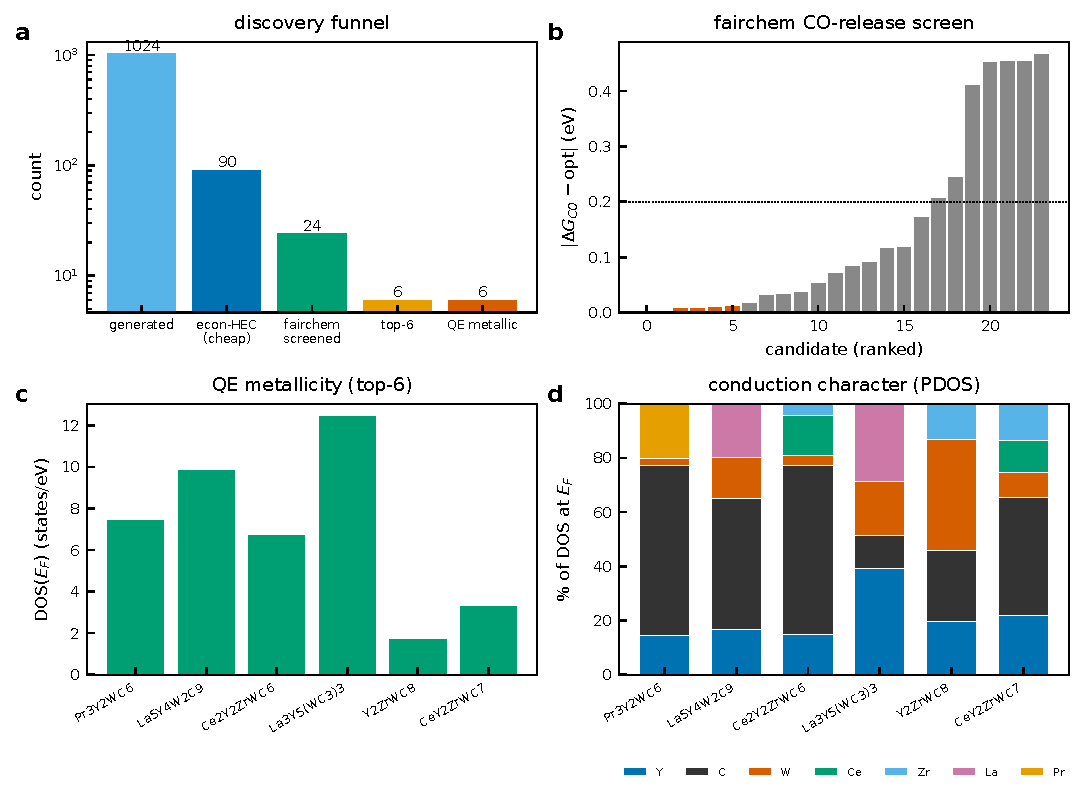
\includegraphics[width=0.92\textwidth]{fig_co2rr_pipeline_summary.pdf}
\caption{End-to-end discovery synthesis. (a) Discovery funnel from 1024 generated structures to 6 DFT-validated metallic candidates.
(b) UMA surface CO-release descriptor of the screened candidates (top six highlighted). (c) Fermi-level DFT density of states of the
top six. (d) Element-projected conduction character (element-wise DOS weight at $\Ef$).}
\label{fig:summary}
\end{figure}

\begin{figure}[t]
\centering
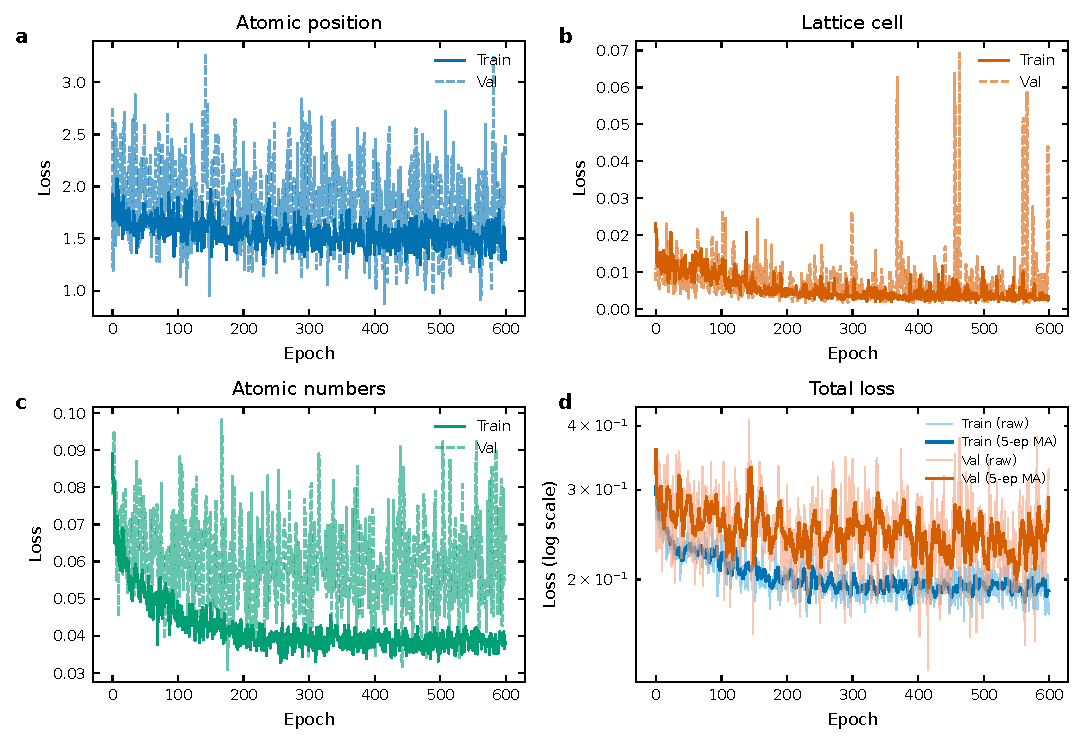
\includegraphics[width=0.78\textwidth]{fig4_composite_economic.pdf}
\caption{Fine-tuning of the economy-conditioned generation model: training/validation loss over 600 epochs and the component-wise (position, lattice,
atom type) losses.}
\label{fig:loss}
\end{figure}

\begin{figure}[t]
\centering
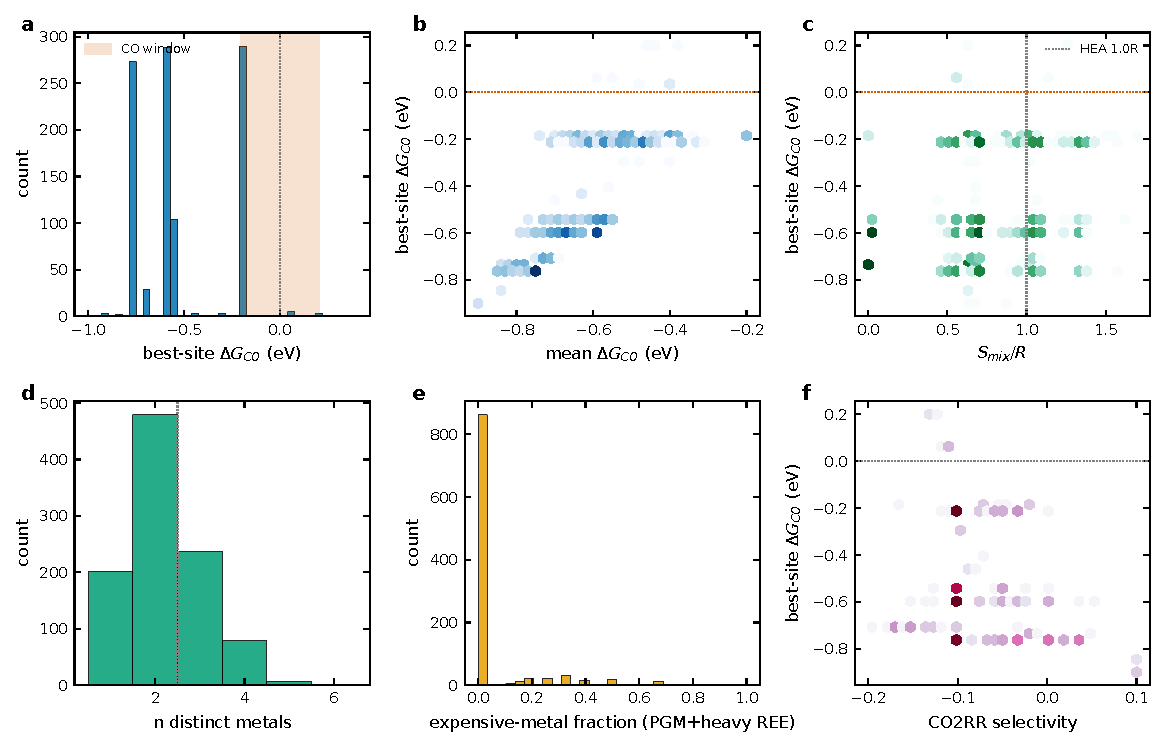
\includegraphics[width=\textwidth]{fig_co2rr_generation_stats.pdf}
\caption{Composition statistics of the generated carbide candidate pool: (a) best-site CO affinity shown together with the CO-release window;
(b,c) descriptor correlations; (d) distribution of metal count; (e) fraction of expensive metals (economy constraint); (f) CO\textsubscript{2}RR
selectivity.}
\label{fig:genstats}
\end{figure}

\begin{figure}[t]
\centering
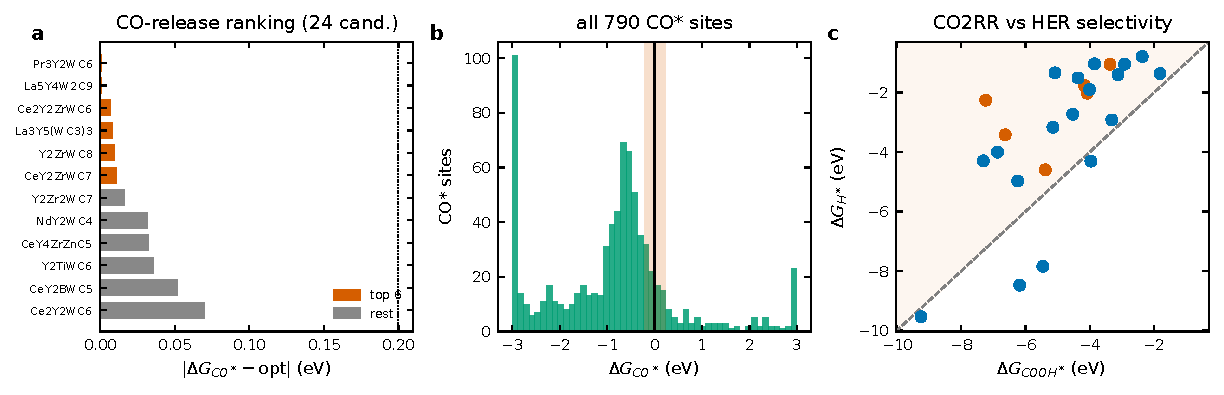
\includegraphics[width=\textwidth]{fig_co2rr_surface_screen.pdf}
\caption{UMA surface screening: (a) candidates ranked by the proximity of their best site to the CO optimum; (b) aggregated $\dGCO$ distribution shown
together with the CO-release window; (c) CO-over-H\textsubscript{2} selectivity ($\dGCOOH$ vs $\dGH$).}
\label{fig:surface}
\end{figure}

\begin{figure}[t]
\centering
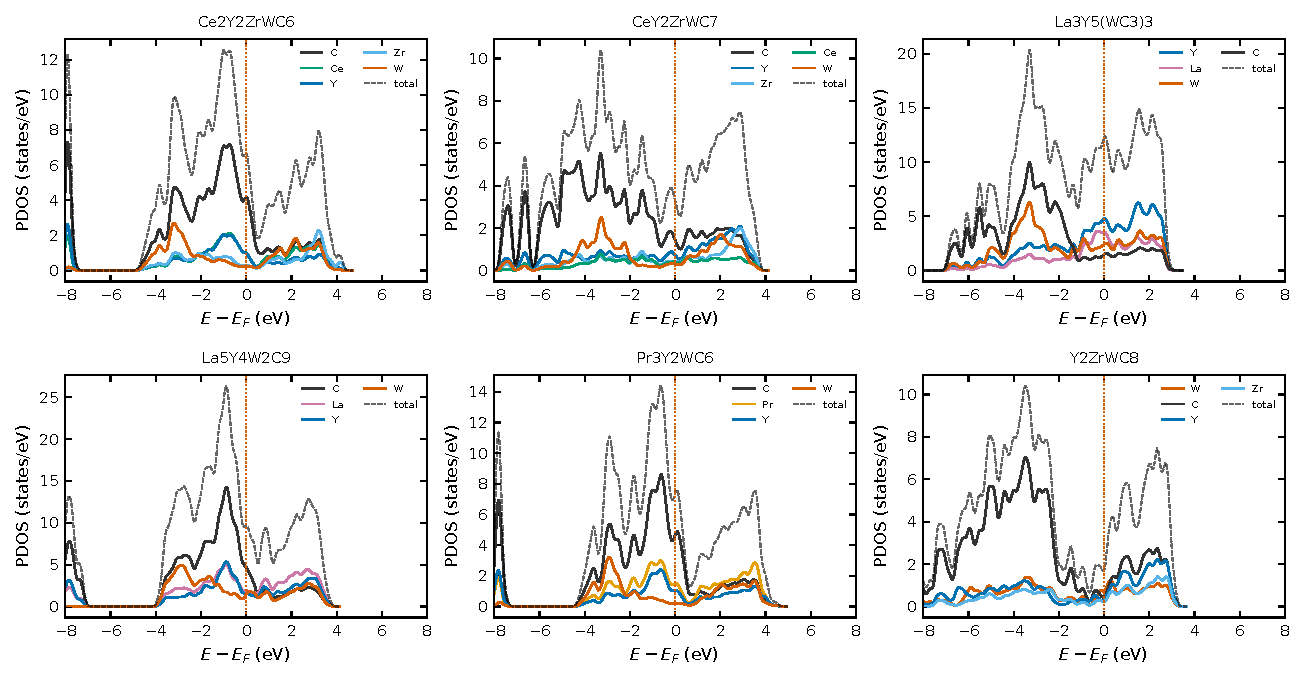
\includegraphics[width=\textwidth]{fig_co2rr_qe_pdos.pdf}
\caption{Element-projected density of states (PDOS) of the six DFT-validated candidates, referenced to $E-\Ef$. The finite states at
$\Ef$ (dashed line) confirm metallicity, and the element-wise decomposition identifies the conduction character.}
\label{fig:pdos}
\end{figure}

\begin{figure}[t]
\centering
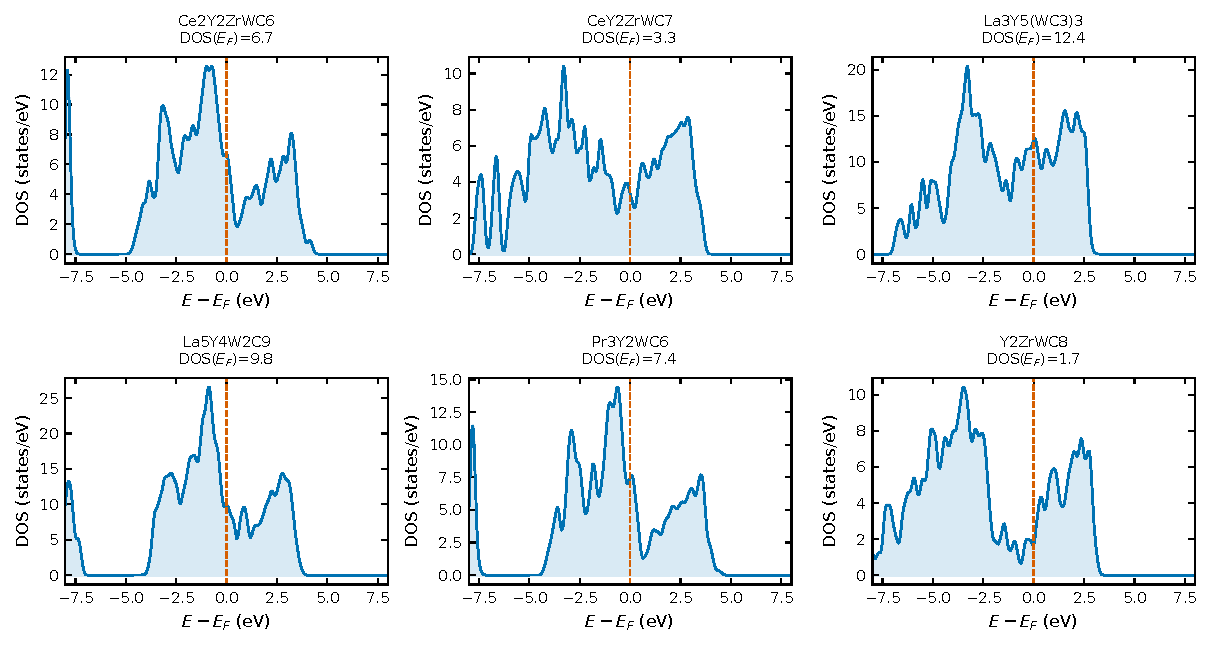
\includegraphics[width=0.9\textwidth]{fig_co2rr_qe_dos.pdf}
\caption{Total density of states of the six candidates near the Fermi level (DFT, PBE).}
\label{fig:dos}
\end{figure}

% =====================================================================
\section{Surface Free Energies and CO\texorpdfstring{$_2$}{2}RR Activity (DFT)}
\label{sec:surf-dft}
For the SQS supercells of the six candidates, we enumerated the symmetrically distinct low-index facets of each crystal structure,
selected the most stable termination for each facet, and then placed $*$CO/$*$COOH/$*$H on every site of the three most active
facets and relaxed them; the resulting geometries (Stage~B, UMA screen) were recomputed as DFT (QE) single-points. In all,
the DFT surface free energies $\dGCO$, $\dGCOOH$, $\dGH$ of \textbf{108 slabs} (6 candidates $\times$ 3 facets $\times$ [clean + 3 adsorbates],
with gas references CO/CO$_2$/H$_2$) were completed (for the computational protocol see
Chapter~\ref{ch:methods}: DFT$/\!/$UMA single-points, $\Gamma$ point, ecut 60/480~Ry, MV smearing).

\paragraph{DFT validation of the MLIP screen.} The DFT and UMA (MLIP) free energies correlate strongly across all 54 (facet, adsorbate)
pairs with Pearson $r=0.973$ (MAE 0.342~eV, RMSE 0.457~eV), with adsorbate-wise MAEs of CO 0.24 /
H 0.30 / COOH 0.49~eV. That is, the \emph{MLIP-level activity ranking is reproduced at the DFT level}. The error is largest for COOH
because of sites at certain low-symmetry facets where $*$COOH overbinds dissociatively ($\dGCOOH \lesssim -2$~eV,
Table~\ref{tab:che}), and DFT partially corrects this unphysical deep well.

\paragraph{Computational hydrogen electrode (CHE) free-energy diagram and limiting potential.} For the two-electron CO$_2\!\to\!$CO path
CO$_2+* \to *$COOH $\to *$CO $\to$ CO(g)$+*$, from the two proton--electron coupled transfer steps
$\Delta G_1=\dGCOOH$ and $\Delta G_2=\dGCO-\dGCOOH$ we define the limiting potential $U_L=-\max(\Delta G_1,\Delta G_2)/e$
(Figure~\ref{fig:che}). \textbf{All six candidates have $\dGCOOH<\dGH$ on their best facet}, i.e.\ CO$_2$
activation is favored over the competing hydrogen evolution reaction (HER), confirming CO selectivity at the DFT level
(Table~\ref{tab:che}). The limiting potentials, however, split clearly into two groups: \emph{CeY$_2$ZrWC$_7$} ($U_L=-0.10$~V) and
\emph{Pr$_3$Y$_2$WC$_6$} ($U_L=-0.21$~V) have a well-defined molecular intermediate that binds $*$COOH moderately and thus a low
overpotential, whereas the remaining four overbind $*$COOH (down to $-7.8$~eV for La$_5$Y$_4$W$_2$C$_9$), making the
$*$COOH$\to*$CO step rate-limiting and giving a large apparent overpotential. For all candidates the potential-determining step (PDS) was
the second reduction step ($*$COOH$\to*$CO). DFT therefore identifies CeY$_2$ZrWC$_7$ and Pr$_3$Y$_2$WC$_6$ as
\emph{low-overpotential CO$_2$RR candidates}.

\begin{table}[t]
\centering
\caption{DFT surface descriptors and CHE limiting potential of each candidate's best facet. $\Delta G$ in eV, $U_L$ in V vs RHE.
All candidates have $\dGCOOH<\dGH$ (CO-selective). PDS is the potential-determining step.}
\label{tab:che}
\small
\begin{tabular}{lcccccc}
\hline
Candidate & Best facet & $\dGCOOH$ & $\dGCO$ & $\dGH$ & $U_L$(DFT) & $U_L$(UMA) \\
\hline
CeY$_2$ZrWC$_7$   & (011)  & $-0.47$ & $-0.37$ & $-0.42$ & $-0.10$ & $-1.80$ \\
Pr$_3$Y$_2$WC$_6$ & (010)  & $-0.63$ & $-0.42$ & $-0.23$ & $-0.21$ & $-0.66$ \\
La$_3$Y$_5$(WC$_3$)$_3$ & (101) & $-1.28$ & $+0.13$ & $-0.34$ & $-1.40$ & $-2.19$ \\
Ce$_2$Y$_2$ZrWC$_6$ & (101) & $-3.12$ & $-0.81$ & $-1.38$ & $-2.31$ & $-2.99$ \\
La$_5$Y$_4$W$_2$C$_9$ & (111) & $-2.40$ & $-0.03$ & $-0.04$ & $-2.37$ & $-2.95$ \\
Y$_2$ZrWC$_8$     & (100)  & $-2.19$ & $+0.22$ & $-0.30$ & $-2.41$ & $-2.50$ \\
\hline
\end{tabular}
\end{table}

\begin{figure}[t]
\centering
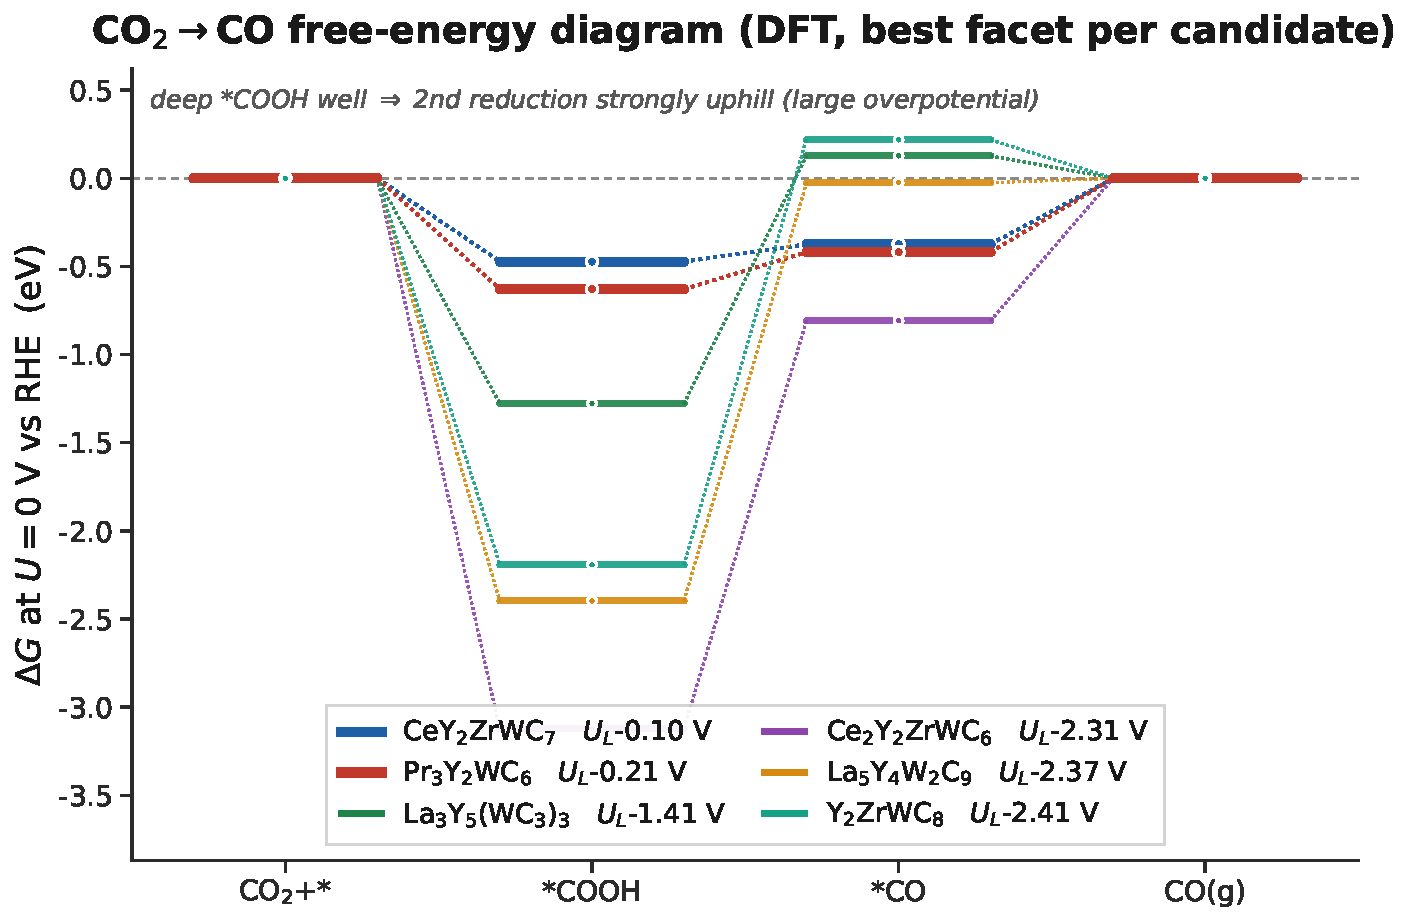
\includegraphics[width=0.92\textwidth]{fig_co2rr_che_diagram.pdf}
\caption{CO$_2\!\to\!$CO computational hydrogen electrode (CHE) free-energy diagrams of the six candidates ($U=0$ vs RHE,
best facet of each candidate). For the low-overpotential candidates (CeY$_2$ZrWC$_7$, Pr$_3$Y$_2$WC$_6$), $*$COOH is a moderate
intermediate state, whereas for the others the $*$COOH deep well makes the second reduction strongly endothermic.}
\label{fig:che}
\end{figure}

\paragraph{$d$-band center and adsorption descriptor.} By projecting each candidate's stored Kohn--Sham wavefunctions onto atomic orbitals
(projwfc), we obtained the $d$-band center $\varepsilon_d$ (relative to $\Ef$) from the transition-metal $d$-projected density of states
(Figure~\ref{fig:dband}). The metal-averaged $\varepsilon_d$ spans from Pr$_3$Y$_2$WC$_6$ ($-0.48$~eV) to
Y$_2$ZrWC$_8$ ($-1.46$~eV), and element-wise, W has the deepest center ($-1$ to $-2.3$~eV) while the rare-earth
5$d$ and Zr are closer to $\Ef$. Consistent with the $d$-band model, candidates whose center is closer to $\Ef$ (higher $\varepsilon_d$)
tend to bind CO more strongly, linking the conduction character to the adsorption descriptor.

\begin{figure}[t]
\centering
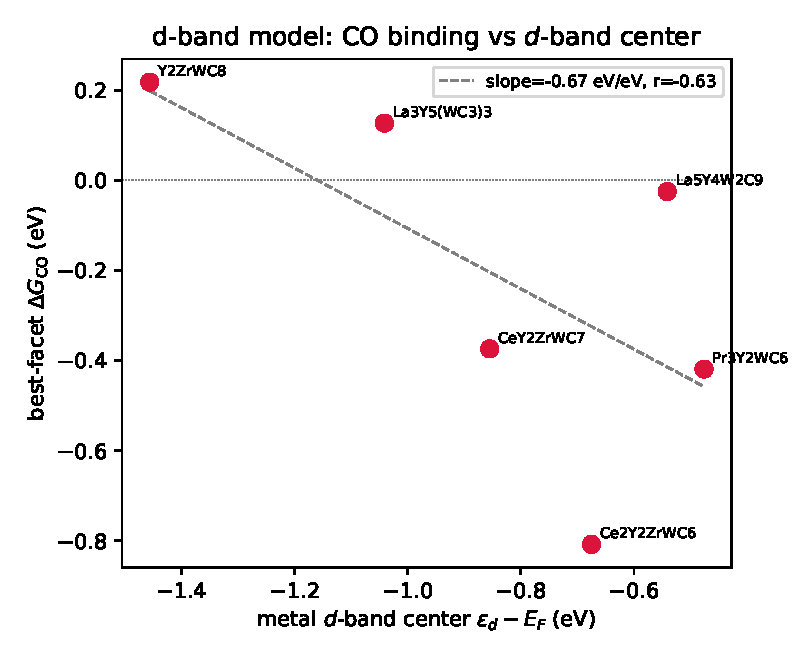
\includegraphics[width=0.62\textwidth]{fig_co2rr_dband_vs_dGCO.pdf}
\caption{Metal $d$-band center $\varepsilon_d-\Ef$ vs best-facet $\dGCO$. A higher $d$-band tends to give stronger CO binding
(trend line), linking conduction character and adsorption.}
\label{fig:dband}
\end{figure}

% =====================================================================
\section{Formation Energies and Convex-Hull Stability (DFT + Materials Project)}
\label{sec:hull}
The bulk formation energies of the six candidates were computed from elemental references at the same QE-PBE level (W bcc, Zr/Y hcp, La/Ce/Pr fcc,
C diamond; vc-relax), and the convex hull was constructed from competing phases in the same chemical space (Materials Project GGA entries,
including all subsystems) to evaluate the above-hull energy $E_{\mathrm{hull}}$ (Table~\ref{tab:hull}). Owing to elemental-reference cancellation,
the difference between the QE and MP (VASP) formation energies is largely removed, and the residual is estimated at the
$\sim$0.1~eV/atom level. The $E_{\mathrm{hull}}$ of the six candidates is $+0.15$ to $+0.36$~eV/atom, which is
\emph{metastable} on a 0~K enthalpy basis --- typical of high-entropy carbides (entropy-stabilized materials, not enthalpic ground states).
The stabilization from the ideal configurational entropy, $-T\Delta S_{\mathrm{mix}}$, is
$-0.05$ to $-0.10$~eV/atom at 1800~K, which reduces the hull distance but by itself does not fully cancel it
(crossover temperature $T^\ast\approx 3000$ to $12000$~K); the actual synthesizability therefore depends jointly on vibrational entropy, non-ideal
mixing enthalpy, \emph{kinetic trapping} by high-temperature quenching, and the methodological uncertainties above.
In short, these ML-generated candidates are metastable phases whose synthesizability is not self-evident, which directly motivates
the synthesis and phase-purity tests (XRD/XPS) of Chapter~\ref{ch:experiment}.

\begin{table}[t]
\centering
\caption{DFT formation energies (QE elemental references), above-hull energy relative to the MP convex hull, and ideal configurational-entropy
stabilization. $E_f, E_{\mathrm{hull}}$ in eV/atom. $T^\ast$ is the temperature at which the ideal entropy cancels the hull distance.}
\label{tab:hull}
\small
\begin{tabular}{lcccc}
\hline
Candidate & $E_f$(QE) & $E_{\mathrm{hull}}$ & $-T\Delta S_{\mathrm{mix}}$(1800\,K) & $T^\ast$(K) \\
\hline
La$_3$Y$_5$(WC$_3$)$_3$ & $-0.087$ & $+0.154$ & $-0.091$ & 3050 \\
La$_5$Y$_4$W$_2$C$_9$   & $-0.024$ & $+0.191$ & $-0.088$ & 3890 \\
CeY$_2$ZrWC$_7$         & $-0.118$ & $+0.223$ & $-0.086$ & 4660 \\
Pr$_3$Y$_2$WC$_6$       & $+0.046$ & $+0.265$ & $-0.078$ & 6080 \\
Ce$_2$Y$_2$ZrWC$_6$     & $-0.067$ & $+0.309$ & $-0.103$ & 5390 \\
Y$_2$ZrWC$_8$           & $+0.072$ & $+0.360$ & $-0.054$ & 12040 \\
\hline
\end{tabular}
\end{table}

% =====================================================================
\section{Refined Validation (Stage C): DFT Relaxation and $k$-Convergence of Top Candidates}
\label{sec:stagec}
The surface free energies presented so far are DFT single-points on UMA-relaxed geometries (DFT$/\!/$UMA, $\Gamma$). For the two most
active candidates (CeY$_2$ZrWC$_7$, Pr$_3$Y$_2$WC$_6$), we refined the headline results by \emph{full ionic relaxation}
(GPU QE, bottom half fixed, $\Gamma$) of the clean slab, $*$CO, $*$COOH, and $*$H on their active facet.

\paragraph{$k$-point convergence.} The symmetry-free $\sim$50-atom slabs cannot run with $k>\Gamma$ on 16~GB of VRAM, but
$\Delta G$ is a difference at the same cell and same $k$, so finite-$k$ errors cancel. On a 36-atom slab, the $\Gamma$ vs
$2{\times}1{\times}1$ difference in adsorption free energy is $\Delta G_{\rm CO}$ 0.01~eV and $\Delta G_{\rm COOH}$ 0.11~eV; even though
the absolute slab energy shifts by $\sim$0.7~eV, the difference is stable, justifying the $\Gamma$-level $\Delta G$.

\paragraph{Relaxation refines the top ranking.} Full relaxation confirmed that \textbf{the low overpotential of CeY$_2$ZrWC$_7$ is robust}:
$\Delta G_{\rm CO}=-0.09$~eV (nearly perfect thermoneutrality; improved by relaxation from the single-point $-0.37$),
$U_L=-0.15$~V (a 0.05~V shift from the single-point $-0.10$). By contrast, \textbf{the single-point activity of Pr$_3$Y$_2$WC$_6$ was not
robust}: upon relaxation the $*$COOH on the active facet \emph{dissociates} (in the relaxed geometry one C--O bond breaks to 3.3~\AA,
decomposing into $*$CO$+*$O), falling into a deep well of $\Delta G_{\rm COOH}=-3.66$~eV and worsening $U_L$ to $-3.1$~V. That is,
the low single-point $U_L$ of Pr$_3$Y$_2$WC$_6$ was an artifact of the UMA geometry. Both candidates show a tendency for $*$COOH dissociation,
but in CeY$_2$ZrWC$_7$ the decomposition products bind moderately, so activity is preserved. Therefore \emph{a $\Delta G_{\rm CO}$ that is
robust to relaxation is the reliable activity descriptor}, and by this criterion \textbf{CeY$_2$ZrWC$_7$ ($\Delta
G_{\rm CO}\!=\!-0.09$~eV) emerges as the uniquely ideal CO-evolution candidate}. The microscopic pathway and microkinetics of
$*$COOH dissociation are subjects for future work.

% =====================================================================
\section{Solid-Solution Supercells and Ongoing Calculations}
\label{sec:outstanding}
In Stage A$'$ (Chapter~\ref{ch:methods}) the special quasirandom structures of the high-entropy shortlist were built as explicit disordered
supercells on rocksalt and hexagonal frameworks (metal-sublattice pair-correlation error minimized), and they are the substrates of the surface
study above (Section~\ref{sec:surf-dft}). Since the \emph{final deliverables of this work are the three Ti-based rocksalt carbides that pass all four
design axioms A1--A4} (hec3-MoTiZr/CrTiV/CrTiZr), we here summarize the \textbf{first-principles validation status of these three}.

\paragraph{Completed validation (three final carbides).}
\begin{itemize}[nosep]
\item \textbf{Dual-objective surface free energies and limiting potential}: per-facet DFT$/\!/$UMA confirms simultaneous CO evolution
($|\dGCO|<0.3$) and H repulsion ($\dGH>0$) and yields $U_L$ (Table~\ref{tab:dual}, Figure~\ref{fig:summaryB}b).
\item \textbf{Full relaxation of the representative candidate}: hec3-MoTiZr (100) was fully relaxed with GPU DFT, reconfirming selectivity
($\dGH\!=\!+0.57$; CO binds weakly ontop Mo and is released) and correcting $U_L$ to $-0.40$~V (Section~\ref{sec:stagec}, Figure~\ref{fig:moTiZr}).
\item \textbf{Convex-hull stability}: from QE-PBE formation energies against the Materials Project hull, all three are more stable than Campaign A
and MoTiZr sits effectively on the hull ($E_{\mathrm{hull}}\!\approx\!-0.02$) (Table~\ref{tab:comp}, Section~\ref{sec:hull}).
\item \textbf{Bulk metallicity and conduction character}: QE bulk DOS/PDOS show all three are metallic (DOS($\Ef$) $21$--$35$~states/eV) and that
the CO-binding group-6 metal (Mo/Cr) dominates the states at $\Ef$ (Figure~\ref{fig:summaryB}c,d).
\item \textbf{Multicarbon branching}: the three fates of $*$CO on the (100) surface (CO release / C1 $*$CHO / C2 $*$OCCO) were computed, and the
C2 coupling is stabilized, consistent with the experimentally observed ethanol (Figure~\ref{fig:cheher}, Section~\ref{sec:tandem}).
\end{itemize}

\paragraph{Remaining first-principles tasks (three final carbides).}
\begin{itemize}[nosep]
\item \tbc{Full relaxation of hec3-CrTiV and CrTiZr (currently single-point) to finalize $U_L$}
\item \tbc{\emph{Coverage-dependent} microkinetics with lateral interactions and a reaction-diffusion local-pH model}
\item \tbc{Projected crystal-orbital (COHP/COOP, LOBSTER) bond-strength analysis to quantify the group-6--CO bond}
\item \tbc{An operating-potential Pourbaix of the \emph{carbide} surface (including lattice stabilization) for oxide-film / OH-poisoning margins}
\item \tbc{Explicit first-principles C--C coupling / ethanol pathway (transition states and barriers)}
\end{itemize}

\paragraph{Role of the Campaign-A (rare-earth) diagnostics.} Separately, for the six rare-earth candidates of Campaign A we also computed the
\emph{dissociative overbinding} of $*$COOH on the active facet (on Pr$_3$Y$_2$WC$_6$ one C--O bond breaks to 3.3~\AA into $*$CO$+*$O,
Section~\ref{sec:stagec}) and the saturated \emph{mean-field coverage} at operating potential ($\theta_{*\mathrm{COOH}}\!\approx\!0.87$--$1.0$).
These are \emph{not} a validation of the final candidates but \textbf{counter-evidence} that the activity-first (unconstrained) search is
mechanically strained as well --- this candidate set is eliminated at the manufacturability gate of the next section
(Section~\ref{sec:ree-stability}), which justifies the manufacturability constraint (A3) of Campaign B. Further computation on the rare-earth
candidates (e.g.\ COHP, coverage-dependent DFT) is therefore \emph{unnecessary}; the remaining tasks focus on the three final carbides above.

% =====================================================================
\section{Manufacturability Gate: Aqueous Oxidation/Leaching of Rare Earths and Active-Site Poisoning}
\label{sec:ree-stability}
The shortlist of Campaign A was selected only for activity, stability, and economy, and was not validated against design axiom
\textbf{A3 (manufacturability)}. This section tests this gate falsifiably with first-principles surface thermodynamics and experimental-thermodynamics Pourbaix analysis. \emph{To state the conclusion up front, the Campaign A candidate pool does not pass this gate} --- and this fact is
the basis for promoting manufacturability to a generation constraint in Campaign B. The shortlist includes light rare earths such as La, Ce, and Pr on the
metal sublattice. These have very high oxygen affinity: their standard reduction potentials for $M^{3+}\!+\!3e^-\!\to\!M$ are La $-2.38$,
Ce $-2.34$, Pr $-2.35$, Y $-2.37$~V (SHE), far more negative than the CO$_2$RR operating window ($\approx -0.5$ to $-1.1$~V vs RHE). That is,
in the \emph{metallic state} the rare earths are thermodynamically strongly inclined toward oxidation/dissolution (e.g.\ $M^{3+}_{(aq)}$ or
$M(OH)_3$/$M_2O_3$). The key question is therefore ``does the stabilization of the carbide lattice offset this driving force and preserve the active site,''
which can be tested falsifiably at three levels of first-principles calculation.

\paragraph{(1) Surface Pourbaix / $*$O, $*$OH coverage (direct test of active-site poisoning).} In the same slab and CHE framework as
$*$CO/$*$COOH/$*$H, we compute the adsorption free energies of $*$O and $*$OH:
$\Delta G_{*\mathrm{OH}}=G_{*\mathrm{OH}}-G_*-(G_{\mathrm{H_2O}}-\tfrac12 G_{\mathrm{H_2}})+eU$,
$\Delta G_{*\mathrm{O}}=G_{*\mathrm{O}}-G_*-(G_{\mathrm{H_2O}}-G_{\mathrm{H_2}})+2eU$.
Taking, at a given $(U,\mathrm{pH})$, the surface species that minimizes the free energy and constructing a \emph{surface Pourbaix diagram}
determines whether, at the operating potential, the surface is clean/$*$H-covered or poisoned by $*$OH/$*$O. In particular, if $*$OH binds
more strongly than $*$CO/$*$COOH at the rare-earth site, active-site poisoning is predicted. \emph{Mitigating factor}:
CO$_2$RR operates at cathodic (reducing) potentials, so oxidation is thermodynamically suppressed (cathodic protection), and the poisoning risk during
normal operation is low; the risk is greatest at open-circuit/startup and under local alkalinization --- the Pourbaix diagram quantifies this
potential/pH dependence.

\emph{$*$O/$*$OH screen (UMA).} We added $*$O and $*$OH as adsorbates to the Stage~B pipeline and screened all facets and all sites of the six candidates
(120--306 sites per candidate). The free energies of the strongest-binding sites are
$\Delta G_{*\mathrm{OH}}(0)=-2.4$ to $-7.0$~eV, $\Delta G_{*\mathrm{O}}(0)=-1.2$ to $-8.8$~eV, far stronger
than $*$CO ($\Delta G_{\rm CO}\!\approx\!0$), showing the large oxygen affinity of these rare-earth-carbide surfaces. This suggests a thermodynamic
\emph{tendency} toward oxidative coverage, but the steady state during actual operation must be judged by a same-facet comparison that includes the reaction intermediate
$*$COOH (see DFT correction below), and it then turns out that $*$COOH prevails rather than oxidation.

\emph{Active-facet same-facet full Pourbaix (DFT, all six candidates completed).} To judge the steady state rigorously, the competing
adsorbates must be compared on the \emph{same facet}, and in particular including the CO$_2$RR reaction intermediate $*$COOH
($\Delta G_{*\mathrm{COOH}}(U)=\Delta G_{*\mathrm{COOH}}(0)+eU$). To this end, on each candidate's
\emph{active facet} (the facet of minimum $U_L$, Table~\ref{tab:che}) we recomputed $*$O/$*$OH with QE (24 slabs, GPU;
La-rich and large slabs with a CPU fallback) and bound them on the same facet as $*$CO/$*$COOH/$*$H. \textbf{On the active facet the
$*$OH/$*$O binding is far weaker than on the worst facet} ($\Delta G_{*\mathrm{OH}}=-0.8$ to $-1.6$~eV, with some
$\Delta G_{*\mathrm{O}}\!\gtrsim\!0$) --- i.e.\ the actual reaction facet has low oxygen affinity. The conclusion of the six-candidate same-facet
Pourbaix (Figure~\ref{fig:pourbaix}): \textbf{at the operating potential ($-0.3$ to $-1.0$~V vs RHE), all six
candidates have the reaction intermediate $*$COOH as the steady state} (6/6 at or below $-0.6$~V, 5/6 at $-0.3$~V; only La$_3$Y$_5$
switches at $-0.6$~V), and $*$O/$*$OH oxidative coverage is confined to a \emph{transient state near open circuit ($\sim\!0$~V)}.
Thus, \emph{under cathodic operating conditions it is not oxidative poisoning but $*$COOH (the operating state) that dominates}, and the earlier
``complete poisoning'' verdict was an artifact of (i) the omission of $*$COOH and (ii) facet mixing. The oxidation risk is real, but its
stage is \emph{startup/open-circuit}, and the substantive axis of candidate differentiation is not oxidation but the $*$COOH binding strength (activity,
Table~\ref{tab:che}). The agreement with UMA is $r=0.74$ (MAE 0.60~eV) on the active facet (weak binding), lower than on the worst facet ($r=0.99$),
which means that MLIP reliability degrades at weakly binding sites, and DFT (the reference) actually gives \emph{even weaker}
binding (lower oxygen affinity). Cross-validation is carried out via the XPS oxidation-state and post-leaching analysis of Chapter~\ref{ch:experiment} and
in-situ FT-IR ($*$COOH/$*$CO bands).

\begin{figure}[t]
\centering
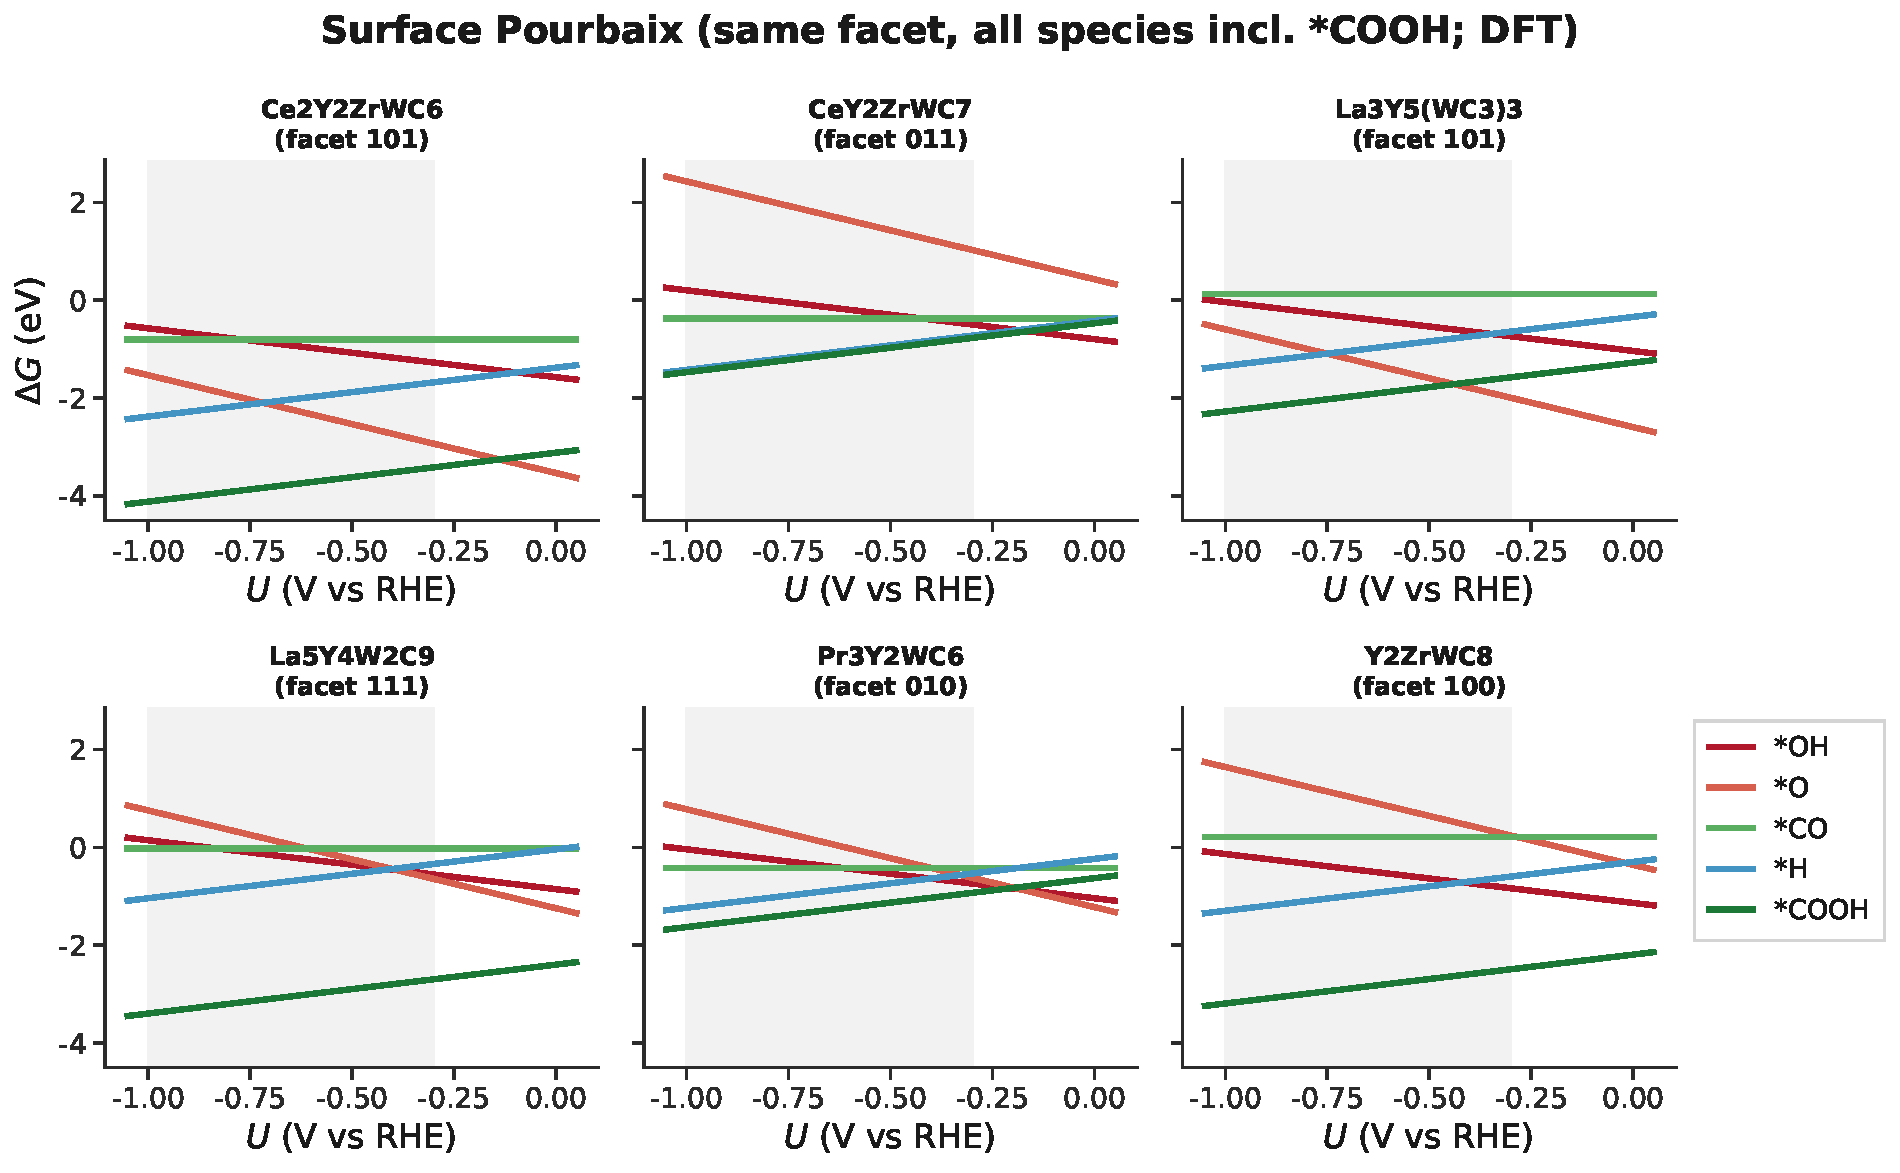
\includegraphics[width=\textwidth]{fig_co2rr_surface_pourbaix_dft.pdf}
\caption{Active-facet same-facet full surface Pourbaix of the six candidates (DFT, including $*$COOH). Potential dependence of each adsorbate's
$\Delta G$; in the operating window (shaded) the species with the lowest $\Delta G$ is the steady state. Across the entire operating potential the reaction intermediate
$*$COOH (green) prevails and the oxidative species ($*$OH/$*$O, red) appear only near open circuit, showing that there is no oxidative poisoning
during operation.}
\label{fig:pourbaix}
\end{figure}

This calculation reuses the Stage~B/Phase~A pipeline (adding $*$O and $*$OH as adsorbates; the
\texttt{-{}-adsorbates OH,O} option of the script \texttt{co\_surface\_screen} and \texttt{61\_surface\_pourbaix.py}).

\paragraph{(2) Bulk Pourbaix / leaching thermodynamics (completed).} Whether the constituent metals remain metallic (immune) at the operating
conditions, passivate as solid oxides/hydroxides, or leach as dissolved ions, was judged with \emph{experimental-thermodynamics}
Pourbaix analysis (the $\Delta G_f$ of aqueous ions and reference oxides from the Materials Project ion reference (Wagman/NBS),
hydroxides from CRC/Wagman tables; Nernst potential/pH dependence computed with pymatgen \texttt{PourbaixDiagram}). Under CO$_2$RR
conditions (pH~7, including local cathodic alkalinization pH~10; $U=0$ to $-1.1$~V vs RHE) the results are (Table~\ref{tab:pourbaix}):
\textbf{no metal is immune (metal-stable) at the operating potential} (except W under cathodic bias). La, Ce, and Zr
\emph{passivate} as hydroxide films, Pr and Y \emph{leach} as ions (though Y passivates at local alkaline pH),
and W dissolves as tungstate (WO$_4^{2-}$) at open circuit but is immune under cathodic bias. That is, the bulk thermodynamics predicts
\emph{oxidation (passivation or leaching) at open-circuit/startup}, consistent with the surface result (operating potential = $*$COOH steady state).
\emph{Note}: this is a \emph{pure-metal} reference and thus a \emph{leaching upper bound} that does not include the carbide lattice stabilization
(the formation energy of Section~\ref{sec:hull}); the actual carbide is more stable. The tabulated-value uncertainty of the hydroxide $\Delta G_f$
($\sim$tens of kJ/mol) also has little effect on the qualitative verdict.

\begin{table}[t]
\centering
\caption{Bulk aqueous Pourbaix (experimental thermodynamics) verdict for the constituent metals. Stable phase in the CO$_2$RR operating window (pH~7)
and at local alkaline pH~10. Immune = metal, passive = solid oxide/hydroxide, leaching = dissolved ion. \emph{Pure-metal reference (leaching upper bound)}.}
\label{tab:pourbaix}
\small
\begin{tabular}{lcc}
\hline
Metal & pH~7 ($0\!\sim\!-1.1$~V RHE) & Local pH~10 \\
\hline
La & Passive (La(OH)$_3$) & Passive \\
Ce & Passive (Ce(OH)$_3$) & Passive \\
Pr & \textbf{Leaching (ion)} & Leaching \\
Y  & \textbf{Leaching (Y$^{3+}$)} & Passive \\
Zr & Passive (Zr(OH)$_4$) & Passive \\
W  & Open-circuit leaching / immune under bias & Immune \\
\hline
\end{tabular}
\end{table}

\paragraph{(3) Explicit surface oxidation / carbon-vacancy formation energies (optional).} We compute, by DFT, the energy of substituting surface C
with O or forming an oxygen overlayer, and the surface carbon-vacancy formation energy, to reinforce the thermodynamics of (1) with the local barrier the lattice
presents against initial oxidation.

Together, these three tests elucidate, quantitatively and falsifiably, the ``risk that even rare earths bound in the lattice cover the active sites by
oxidation/leaching upon exposure to the electrolyte.'' The (1) surface $*$O/$*$OH Pourbaix and (2) bulk leaching Pourbaix above are \emph{completed}
and give a consistent picture: \textbf{at the operating cathodic potential the surface is in the $*$COOH steady state, but at open-circuit/startup
conditions the bulk metal passivates (La, Ce, Zr) or leaches (Pr, Y)}. Experimentally, this is cross-validated by XPS (surface
oxidation state) before and after testing, ICP-MS of the leachate, and the $M$--O bands of in-situ Raman/SEIRAS (Chapter~\ref{ch:experiment}).

% =====================================================================
\section{Campaign B --- Dual Active-Site Design of Acid-Stable Carbides}
\label{sec:campaignB}\label{sec:ree-free}
Campaign B imposes all four design axioms (A1--A4). The decisive differences from Campaign A are twofold --- it internalizes manufacturability (A3)
into the search space, and it strengthens selectivity (A2) into an explicit CO/H \emph{dual active-site} criterion.
The rationale for excluding rare earths rests on \emph{two independent propositions}, and it is important to keep them separate.

\emph{(Rationale 1 --- manufacturability.)} The synthesis route for these carbides metallothermically reduces an oxide precursor with Mg/Ca and then removes the
byproduct oxides (MgO/CaO) by \emph{acid leaching}. In this indispensable leaching step the rare earths dissolve entirely
(the standard reduction potentials of La/Ce/Pr/Y are very negative and their $M^{3+}$ hydration is strong; Section~\ref{sec:ree-stability}), so the
candidate pool of Campaign A becomes \emph{already unmanufacturable at the synthesis stage prior to operation}. This is a \emph{synthesis}
constraint independent of active-site physics. \emph{(Rationale 2 --- non-necessity.)} As shown below, the dual active-site behavior of CO release and H
repulsion is explained by the \emph{valence-electron concentration (VEC)} effect of the transition metals (low VEC = group-4-rich = H repulsion) and requires
no rare earths at all --- indeed, the rare earths (group 3, $f$-electrons) lie outside this VEC-controlled regime. That is, the rare earths must be excluded
on manufacturing grounds and are \emph{simultaneously} unnecessary for active-site design. Since the two rationales hold independently, the exclusion
conclusion survives even if either one is weakened.

\paragraph{Search space and conditioning labels.} Campaign B therefore restricts the metal sublattice to \emph{acid-leaching-tolerant} group-4/5/6
transition metals \{Ti, Zr, Hf, V, Nb, Ta, Cr, Mo, W\} and the nonmetals \{C, B, N\} (a hard whitelist,
\texttt{carbidemattergen/element\_policy.py}), and excludes at the source the rare earths (including Sc and Y), the platinum-group metals, and --- for
\emph{scientific honesty} --- the well-known CO$_2$RR metals \{Cu, Ag, Au, Zn\}. The latter exclusion is a methodological
reason: adding a known CO$_2$RR metal to a carbide support would obscure the generation model's contribution to discovery, so to ensure that the activity
originates from \emph{new carbide chemistry} these must be excluded. For conditioning labels, instead of a literature-based composition surrogate table, we use
\emph{surface labels computed directly with UMA} (the surrogate table is essentially noise, correlating with the UMA labels at $r\!\approx\!0.04$, and so was not adopted).
Because UMA surface labeling is expensive, we narrow the Campaign A carbide set to the acid-stable palette and then re-fine-tune
\textsc{CarbideMatterGen} on a high-quality subset re-labeled with UMA (\textbf{271 training + 34 validation};
the same adapter scheme and hyperparameters, Section~\ref{sec:methods-stageA}). Campaign B's conditioning is thereby grounded directly in surface active-site
physics rather than in a compositional surrogate indicator.

\paragraph{HER competition and hydrogen poisoning: the dual objective.} A CO$_2\!\to\!$CO active site ($\dGCO\!\approx\!0$) often binds H well too,
and since HER and CO evolution compete for the site, activity alone is insufficient. In particular, \textbf{strong H adsorption is
\emph{poisoning} in which $*$H covers the surface and eliminates the sites where CO$_2$ could adsorb}, so the desired condition is a low CO overpotential
and \emph{simultaneously} a high HER overpotential --- i.e.\ the surface must \emph{repel} H ($\dGH>0$). We therefore strengthened the candidate criterion
into a dual objective:
\[
|\dGCO|<0.3~\text{eV (CO evolution, non-poisoning)} \quad\text{and}\quad \dGH>0~\text{(H repulsion, site preservation)}.
\]
$\dGH$ is defined as the \emph{per-facet} physical-site minimum: the global minimum $\dGH$ is an artifact in which a single dissociative/subsurface H
site ($\dGH\!\sim\!-6$~eV) masks an entire facet as H-repelling, so we take the minimum over the physically adsorbed sites, excluding
$|\dGH|>1.5$~eV (dissociation/subsurface), for each facet (\texttt{scripts/63\_perfacet\_dual.py}). This is the requirement that CO evolution and
H repulsion hold on the \emph{same facet}.

\paragraph{DFT dual-objective verdict: three Ti-based carbides.} Recomputing the 15 species that passed the per-facet dual-objective screen as DFT
single-points (DFT$/\!/$UMA, $\Gamma$), \textbf{three satisfy the dual objective}, and all are the (100) facet of Ti-based
three-metal rocksalt carbides (Table~\ref{tab:dual}). The remaining 12 fail by \emph{hydrogen poisoning} with $\dGH<0$ ---
confirming that \emph{H poisoning is the dominant failure mode}. The Nb/Ta/Mo-rich candidates that the generation model selected on the CO-evolution
condition alone released CO but were poisoned by H, whereas the chemistry that repels H was \emph{group-4-rich} (low valence-electron concentration, VEC)
such as Ti+Cr/Mo. Indeed, the metal-averaged VEC of the winners is $\approx\!4.67$ and that of the failures is
$\approx\!5.5$, showing that \textbf{VEC is the physical lever that jointly tunes H repulsion and CO evolution}.

\begin{figure}[t]
\centering
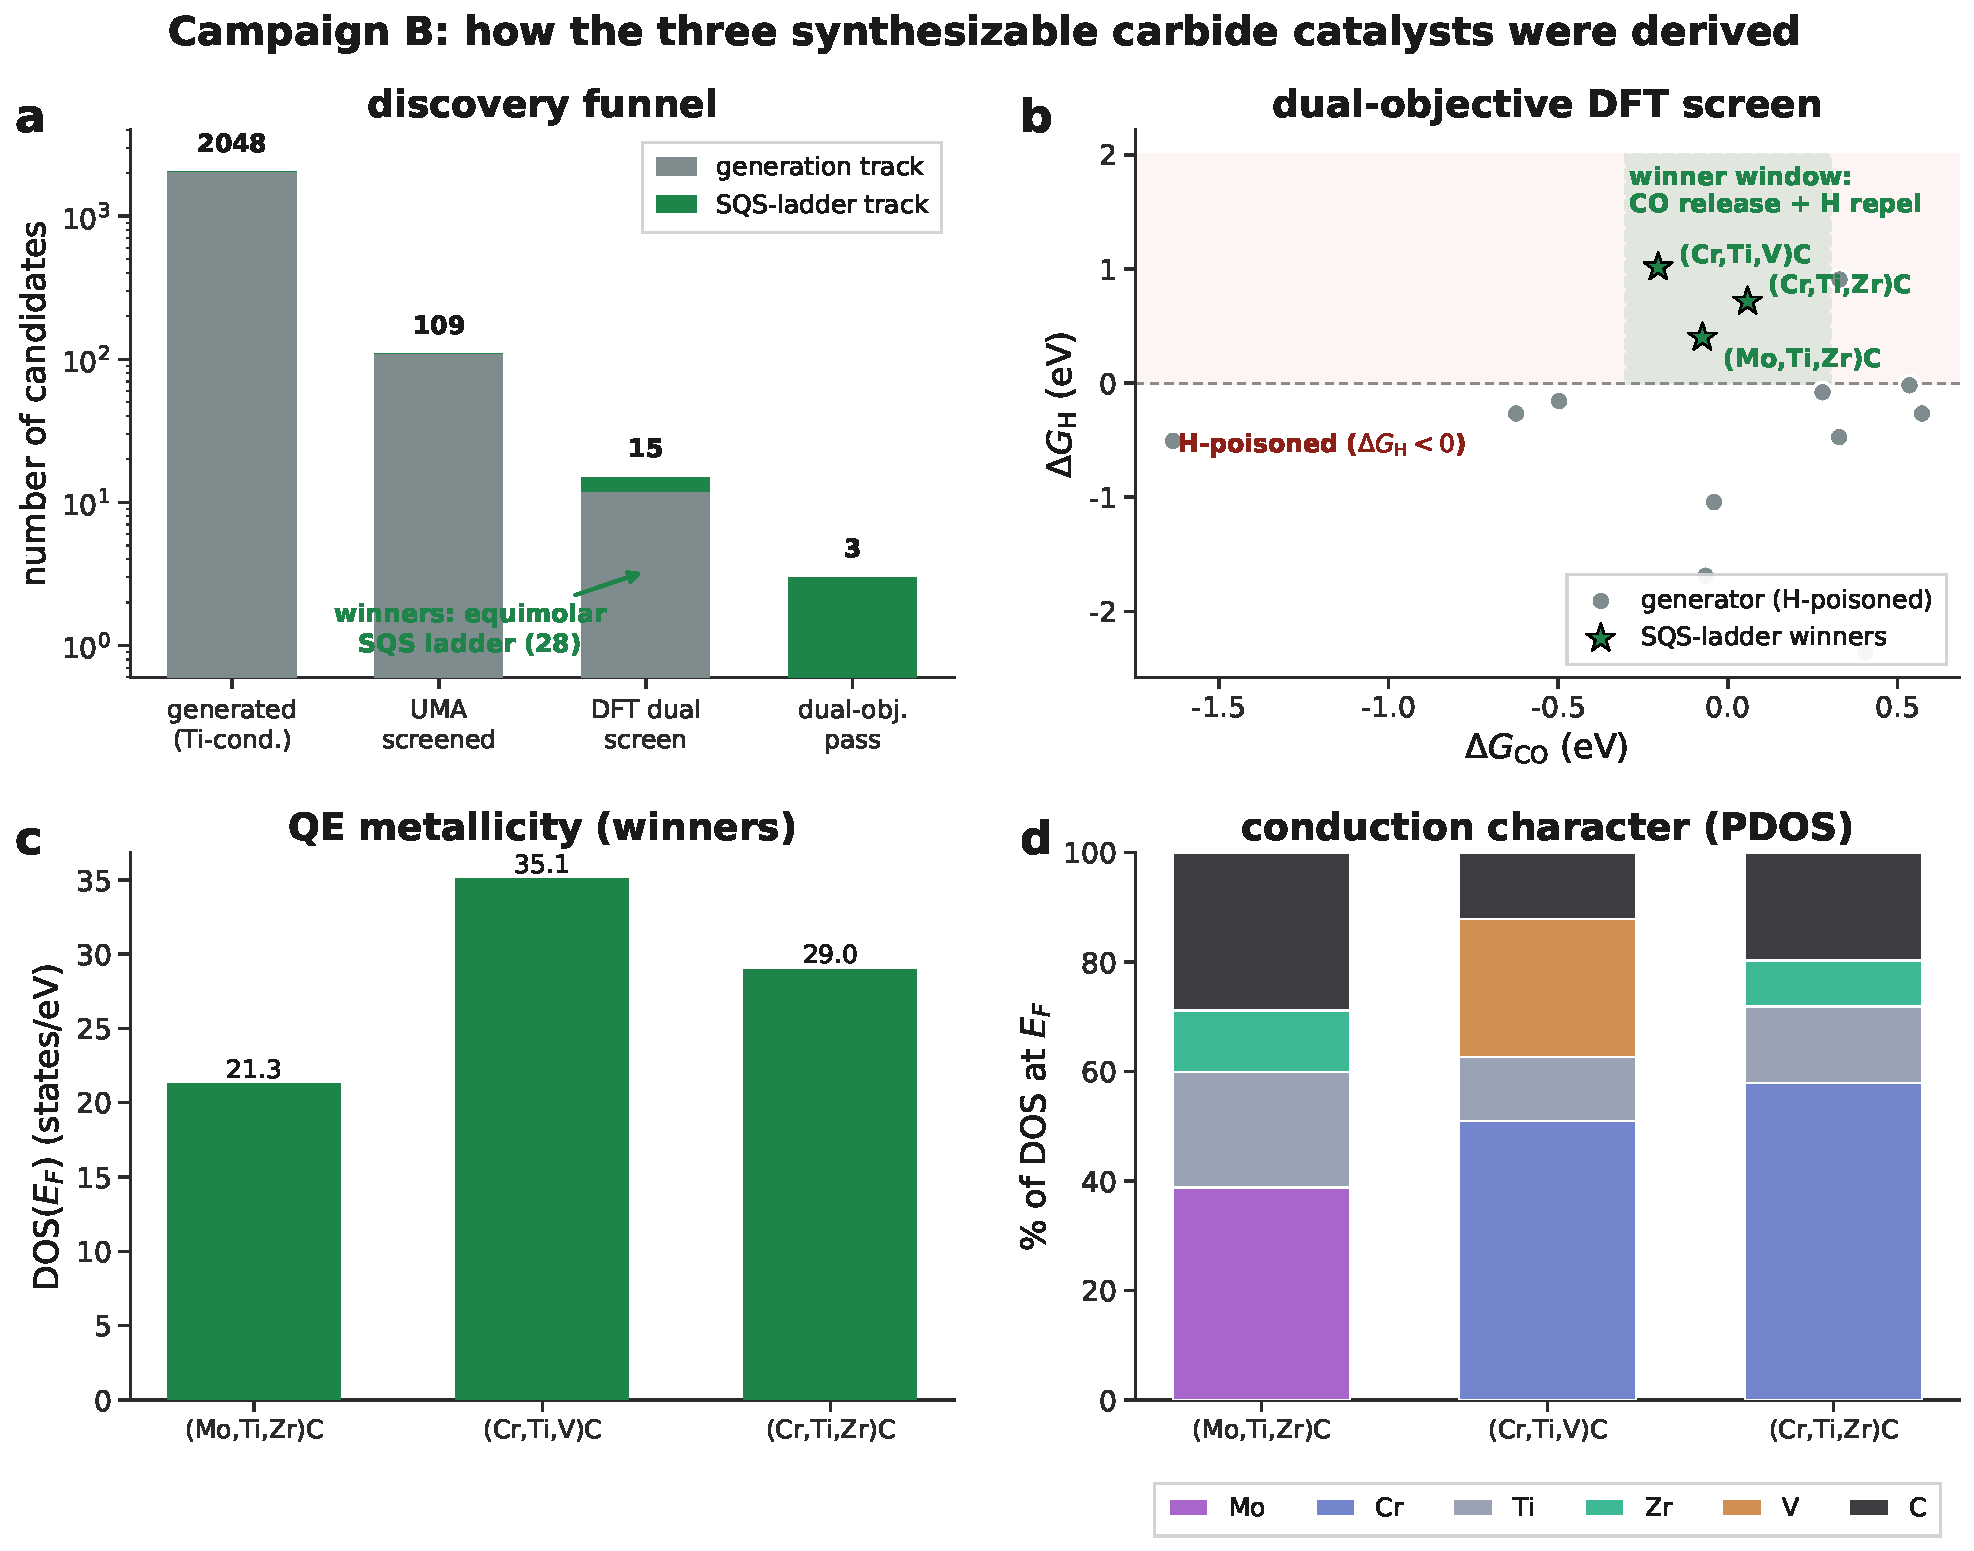
\includegraphics[width=\textwidth]{fig_co2rr_pipeline_summary_B.pdf}
\caption{End-to-end derivation of the Campaign-B candidates --- the carbide analog of
Figure~\ref{fig:summary} (Campaign A). (a) Discovery funnel: 2048 Ti-conditioned generated structures
$\to$ UMA screen $\to$ 15 DFT dual-objective-screened $\to$ 3 that pass. The \emph{generation track}
(grey) sends 12 candidates to DFT that are \emph{all} lost to H-poisoning (0 pass), whereas the 3 winners
come from the \emph{equimolar SQS ladder} (green) --- i.e.\ the generator under-samples the H-repelling
Ti-rich chemistry, so the winners were secured by systematic SQS construction. (b) DFT dual-objective
screen: $\dGCO$ vs $\dGH$. Only the three Ti-based carbides (stars) fall in the winner window
(CO release $|\dGCO|<0.3$ \emph{and} H repulsion $\dGH>0$); the 12 generator candidates are poisoned
($\dGH<0$). (c) QE bulk metallicity DOS($E_F$) of the three winners. (d) Element-projected conduction
character (per-element share of the DOS at $E_F$). Panels (c,d) are at the same computational level as
Figure~\ref{fig:summary}(c,d) (QE bulk SCF $\to$ dos $\to$ projwfc).}
\label{fig:summaryB}
\end{figure}

\paragraph{Composition and structure.} All three candidates are \emph{equimolar three-metal rocksalt monocarbides}
$(M,M',M'')\mathrm{C}$ with metal:carbon $=1:1$ (Table~\ref{tab:comp}): hec3-MoTiZr $=$
$(\mathrm{Mo},\mathrm{Ti},\mathrm{Zr})\mathrm{C}$, hec3-CrTiV $=(\mathrm{Cr},\mathrm{Ti},\mathrm{V})\mathrm{C}$,
hec3-CrTiZr $=(\mathrm{Cr},\mathrm{Ti},\mathrm{Zr})\mathrm{C}$. The metal counts of the 64-atom SQS (100) slab are
$11{:}11{:}10$, approximating equimolarity (e.g.\ Mo$_{11}$Ti$_{11}$Zr$_{10}$C$_{32}$). The metal sublattices are all
acid-leaching-stable group-4/5/6 transition metals, so they satisfy the campaign's design constraint (A3).

\begin{table}[t]
\centering
\caption{Composition/structure and synthesizability indicators of the Campaign B final candidates. VEC is the metal-averaged valence-electron count (group 4/5/6
$=4/5/6$). ``Acid-stable'' denotes survival of acid leaching (A3). $E_{\mathrm{hull}}$ (eV/atom) is computed from
QE-PBE formation energies against the Materials Project convex hull (GGA/GGA+U): all three are more stable than
Campaign A (REE, $+0.15\!\sim\!+0.36$), and MoTiZr is effectively on the hull ($\approx\!0$).}
\label{tab:comp}
\setlength{\tabcolsep}{3pt}\footnotesize
\begin{tabular}{llcccccc}
\hline
Candidate & \shortstack{Ideal\\comp.} & \shortstack{Slab\\(64 atoms)} & Structure & \shortstack{Active\\facet} & VEC & \shortstack{Acid-\\stable} & $E_{\mathrm{hull}}$ \\
\hline
hec3-MoTiZr & $(\mathrm{Mo,Ti,Zr})\mathrm{C}$ & Mo$_{11}$Ti$_{11}$Zr$_{10}$C$_{32}$ & Rocksalt $MC$ & (100) & 4.67 & $\bigcirc$ & $-0.02$ \\
hec3-CrTiV  & $(\mathrm{Cr,Ti,V})\mathrm{C}$  & Cr$_{11}$Ti$_{11}$V$_{10}$C$_{32}$  & Rocksalt $MC$ & (100) & 5.00 & $\bigcirc$ & $+0.05$ \\
hec3-CrTiZr & $(\mathrm{Cr,Ti,Zr})\mathrm{C}$ & Cr$_{11}$Ti$_{11}$Zr$_{10}$C$_{32}$ & Rocksalt $MC$ & (100) & 4.67 & $\bigcirc$ & $+0.10$ \\
\hline
\end{tabular}
\end{table}

\begin{table}[t]
\centering
\caption{Summary of the DFT active sites and free energies of the Campaign B final candidates. $\Delta G$ in eV, $U_L$ in V vs RHE.
The active facet is (100) for all; all three simultaneously satisfy CO evolution ($|\dGCO|<0.3$) and H repulsion ($\dGH>0$). The potential-determining
step (PDS) is $*$COOH formation ($\mathrm{CO_2}\!+\!*\!\to\!{*}\mathrm{COOH}$) for all three candidates.}
\label{tab:dual}
\footnotesize\setlength{\tabcolsep}{4pt}
\begin{tabular}{llcccccl}
\hline
Candidate & Method & $*$CO site & $\dGCO$ & $\dGCOOH$ & $\dGH$ & $U_L$ & Verdict \\
\hline
hec3-MoTiZr & single-point & Mo ontop (weak) & $-0.08$ & $+0.13$ & $+0.40$ & $-0.13$ & CO-selective \\
hec3-MoTiZr & \textbf{relaxed} & Mo ontop (released) & $+0.18$ & $+0.39$ & $+0.57$ & $-0.40$ & \textbf{CO-sel.\ (conf.)} \\
hec3-CrTiV  & single-point & Cr ontop & $-0.20$ & $+0.73$ & $+1.01$ & $-0.73$ & CO-selective \\
hec3-CrTiZr & single-point & Cr ontop & $+0.06$ & $+0.72$ & $+0.71$ & $-0.72$ & CO-selective \\
\hline
\end{tabular}
\end{table}

\paragraph{Active sites.} Looking at the nearest metal to the adsorbate (minimum-image distance) in the relaxed/screened geometries reveals a clear pattern:
$*$CO binds \emph{ontop a group-6 metal} in all three candidates (Cr in CrTiV $\sim\!1.9$~\AA, Cr in CrTiZr $\sim\!2.0$~\AA, Mo in MoTiZr $\sim\!2.1$~\AA).
The binding strength differs, however: MoTiZr binds weakly ($\dGCO\!=\!+0.18\!>\!0$) and thus \emph{releases} CO, whereas CrTiV binds strongly ($\dGCO\!=\!-0.20$) and holds it. $*$H sits ontop/bridge on a metal
(e.g.\ on Mo at $1.76$~\AA in MoTiZr, on a Zr bridge $\sim\!2.1$~\AA in CrTiZr) but is unfavorable in free energy, so its
coverage is suppressed. That is, CO binding is tuned by the group-6 metal and H repulsion by the group-4-rich (low-VEC) framework. The (100)-surface CO active sites of the three
candidates are shown in Figure~\ref{fig:sites}.

\begin{figure}[t]
\centering
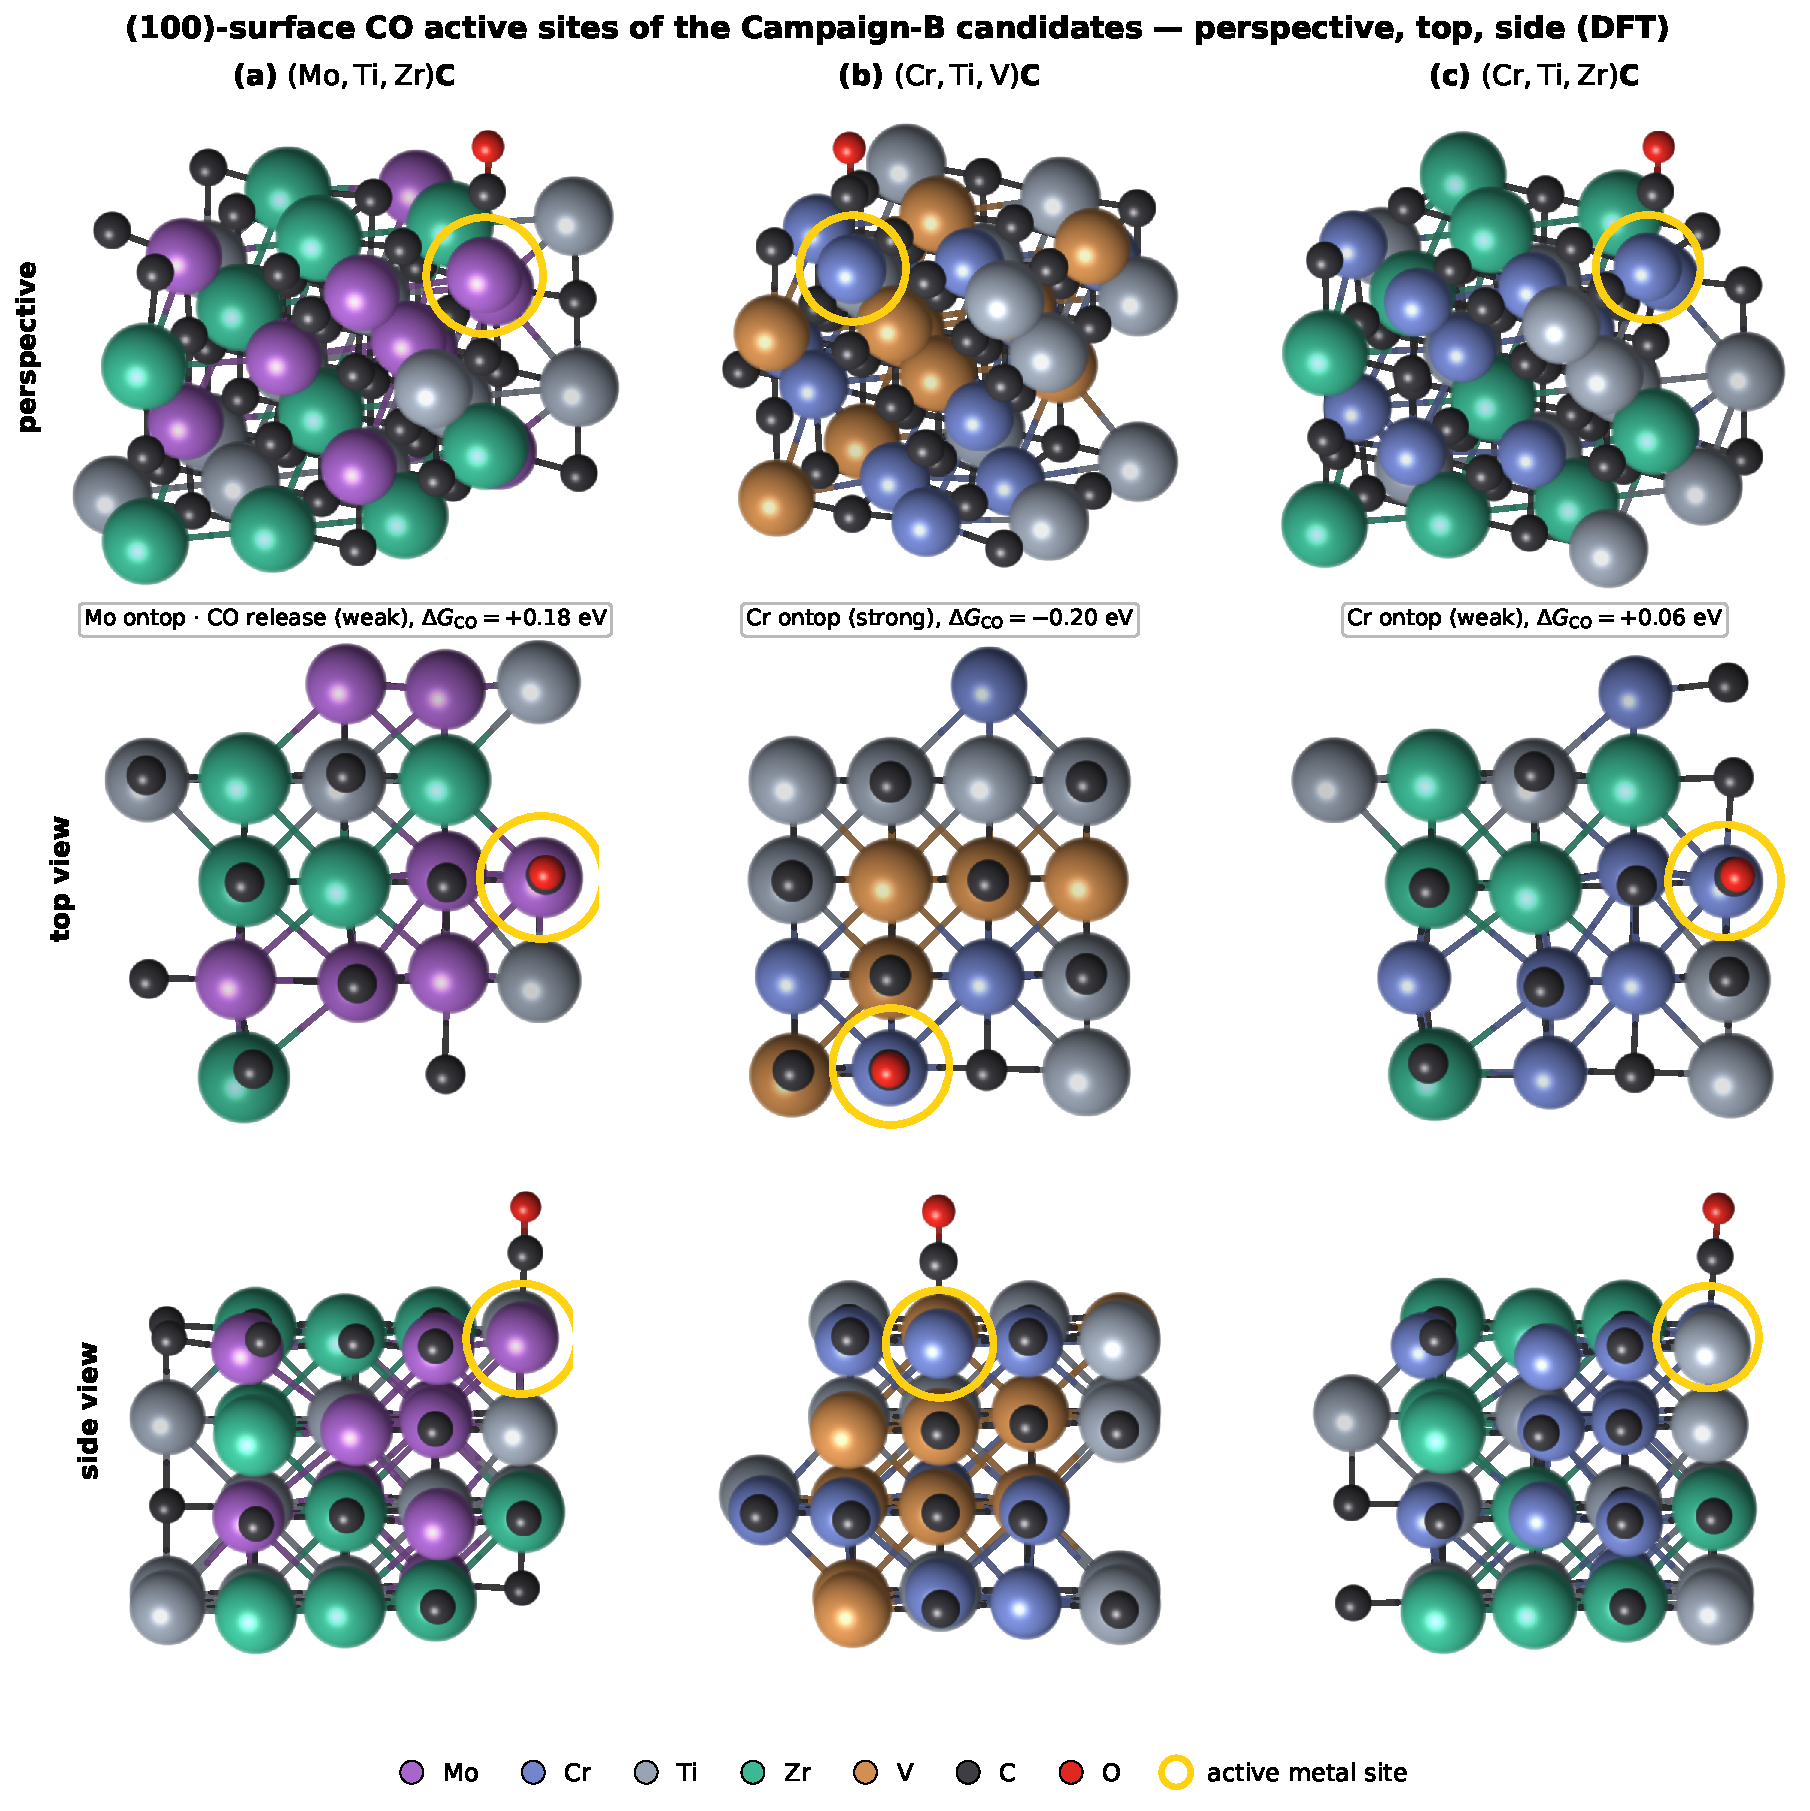
\includegraphics[width=\textwidth]{fig_co2rr_active_sites_en.pdf}
\caption{(100)-surface CO active sites of the three Campaign B final candidates (DFT relaxed/screened geometries). \textbf{Columns} are the three
candidates; \textbf{rows} are the perspective (3D), top view (looking straight down), and side view (from the front). In each panel the yellow
ring marks the nearest (active) metal site of the adsorbed CO. The top view places the CO oxygen (red) directly over the active metal, and the
side view shows the CO standing vertically above the surface in an \emph{ontop} geometry, making the active location unambiguous.
(a) $(\mathrm{Mo,Ti,Zr})$C binds CO weakly \emph{ontop Mo} ($\sim\!2.1$~\AA) but, since $\dGCO\!=\!+0.18\!>\!0$, \emph{releases} it (relaxed).
(b) $(\mathrm{Cr,Ti,V})$C and (c) $(\mathrm{Cr,Ti,Zr})$C bind CO at the \emph{Cr ontop} site
($\sim\!1.9$--$2.0$~\AA). For all three candidates, CO binding/release is tuned by the group-6 (Cr/Mo) site. See the legend for atom colors;
the active facet is (100) for all.}
\label{fig:sites}
\end{figure}

\paragraph{Free-energy diagrams: HER suppressed, CO$_2$RR favored.} The CO$_2$RR (CO$_2\!\to\!$CO)
and HER free-energy diagrams of the three candidates are shown together in Fig.~\ref{fig:cheher}. The
CO$_2$RR pathway is accessible at the applied limiting potential $U_L$, whereas the HER intermediate
$*$H sits \emph{positive} in free energy for all three candidates ($\dGH\!=\!+0.57\!\sim\!+1.01$~eV),
so *H coverage is suppressed --- i.e.\ \emph{the same surface suppresses HER while favoring CO$_2$RR}.
CO is, however, the \emph{gateway intermediate}: further reduction beyond CO to multicarbon (C$_{2+}$)
products such as ethanol requires calculation of the C--C coupling pathway (Section~\ref{sec:tandem})
and is therefore only indicated conceptually here (grey dashed) --- the full CO$_2\!\to\!$ethanol diagram
is future work (the earlier CO$_2\!\to\!$CO diagram, Fig.~\ref{fig:che}, stops at CO for the same reason).

\begin{figure}[t]
\centering
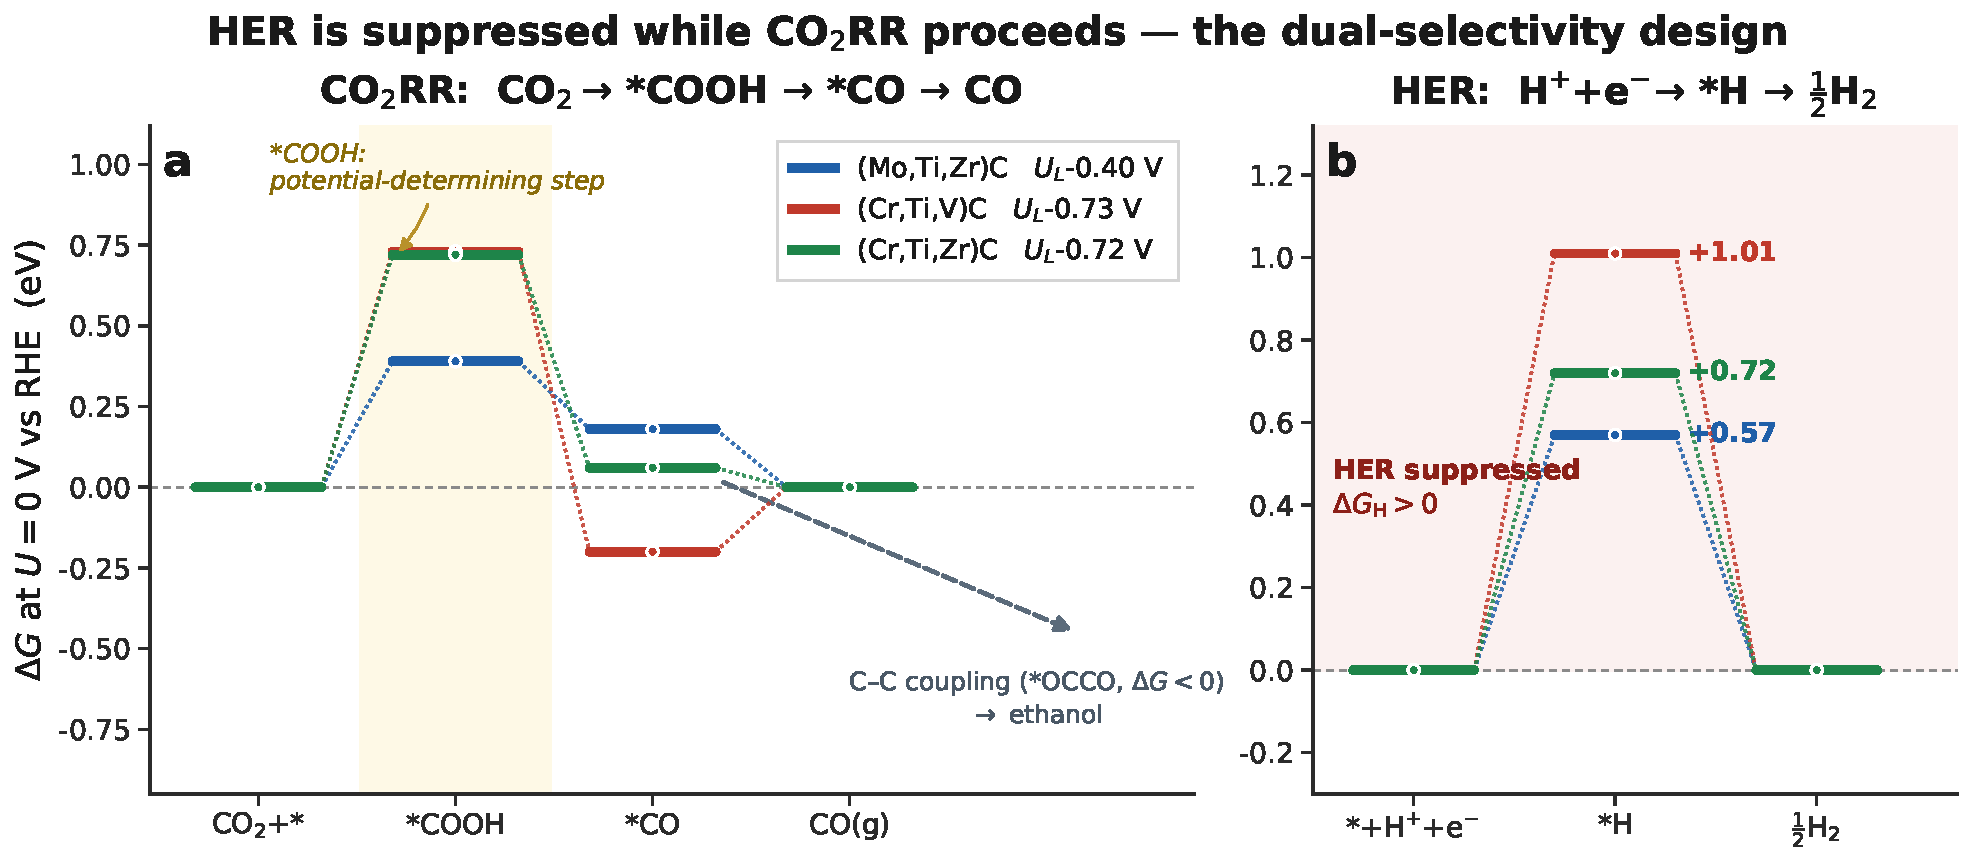
\includegraphics[width=\textwidth]{fig_co2rr_che_her_en.pdf}
\caption{Free-energy diagrams of the three Campaign-B final candidates ($U=0$ vs RHE). (a) CO$_2$RR:
CO$_2\!\to\!*$COOH$\!\to\!*$CO$\!\to\!$CO; the potential-determining step is $*$COOH formation for all
three. Route beyond $*$CO to ethanol (C$_{2+}$): the first C--C-coupling intermediate ($*$OCCO,
C--C$\approx$1.5~\AA, $\Delta G<0$) was computed and shows the C2 (ethanol) route is favored (C1 $*$CHO is
endergonic; Section~\ref{sec:tandem}); the grey dashed arrow denotes that the \emph{full} downstream pathway
(transition states / complete route) is still conceptual. (b) HER:
H$^+\!+\!$e$^-\!\to\!*$H$\!\to\!\tfrac12$H$_2$; the $*$H level is positive ($\dGH>0$) for all three, so
HER is suppressed (shaded region). The top of the $y$-axis is matched across panels so the CO$_2$RR
rate-limiting level ($*$COOH) and the HER $*$H height can be compared directly. hec3-MoTiZr is relaxed;
the other two are single-point.}
\label{fig:cheher}
\end{figure}

\paragraph{Full relaxation of the lead candidate: selectivity robust, limiting potential corrected.} For the active (100) facet of the headline candidate hec3-MoTiZr,
we fully ionically relaxed the clean slab, $*$CO, $*$COOH, and $*$H (GPU QE, bottom half fixed,
$\Gamma$). For the same reason as in Section~\ref{sec:stagec}, the symmetry-free 64-atom-class slab cannot run a
$2{\times}2{\times}1$ $k$-mesh (16.4~GB) on 16~GB of VRAM, so it was relaxed at $\Gamma$, and the cancellation of finite-$k$ error, since $\Delta G$ is a same-cell difference,
was verified earlier. \textbf{The core selectivity claim is robust to relaxation}:
$\dGH=+0.57$~eV, which is actually \emph{strengthened} relative to the single-point ($+0.40$), confirming that the H repulsion is not a geometric artifact,
and $\dGCO=+0.18$~eV, so CO is still weakly bound and desorbs (CO-selective = YES). By contrast, \textbf{the limiting potential is corrected}:
upon relaxation, $*$COOH formation ($\dGCOOH=+0.39$~eV) becomes endothermic and thus the potential-determining step, and
$U_L=-0.40$~V (single-point $-0.13$) worsens. That is, full relaxation \emph{confirms the selectivity} while \emph{correcting the apparent
activity}, revealing that the single-point DFT$/\!/$UMA underestimated the $*$COOH barrier --- demonstrating exactly the value of relaxation
validation. The relaxed final structure (Figure~\ref{fig:moTiZr}) shows the dual selectivity directly through geometry:
after relaxation $*$CO remains weakly bound \emph{ontop} Mo ($\sim\!2.1$~\AA) but, since $\dGCO\!=\!+0.18\!>\!0$, is thermodynamically \emph{released} rather than poisoning the surface, while
$*$H adsorbs on the surface ($\sim\!1.7$~\AA) but is unfavorable in free energy ($\dGH\!=\!+0.57$~eV), keeping its coverage low.

\begin{figure}[t]
\centering
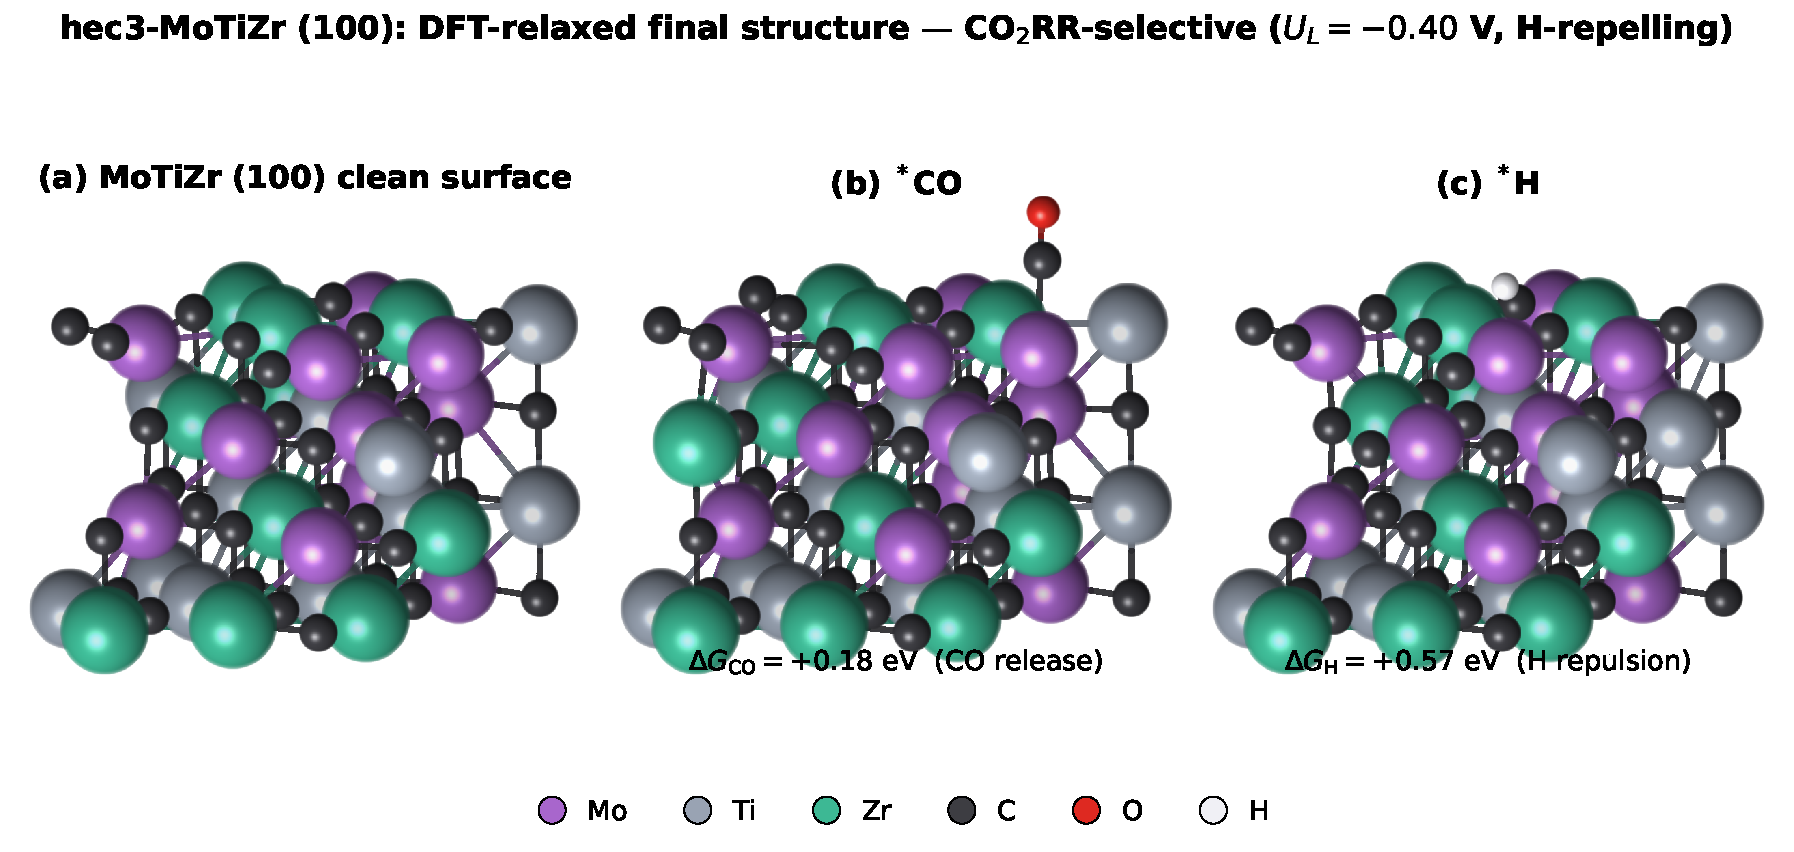
\includegraphics[width=\textwidth]{fig_co2rr_moTiZr_structure_en.pdf}
\caption{DFT fully relaxed final structure of the headline candidate \textbf{hec3-MoTiZr (100)} (SQS 64-atom slab,
bottom half fixed, $\Gamma$). (a) clean surface, (b) $*$CO, (c) $*$H. The dual objective is revealed geometrically:
after relaxation $*$CO stays weakly bound \emph{ontop} Mo ($\sim\!2.1$~\AA) but is \emph{released} thermodynamically ($\dGCO=+0.18$~eV, weak binding), while $*$H
adsorbs on the surface but is unfavorable in free energy ($\dGH=+0.57$~eV, H repulsion), suppressing its coverage. That is, the surface leaves the
CO$_2$RR intermediate site vacant while suppressing HER ($U_L=-0.40$~V vs RHE, CO$_2$RR-selective).
Atom colors: Mo purple, Ti gray, Zr green, C dark gray, O red, H white. Coordinate files are
\texttt{results\_cif/MoTiZr\_*.cif}.}
\label{fig:moTiZr}
\end{figure}

\paragraph{Retargeting the generator: low-VEC conditioning drives discovery.} The three winners above came from the high-entropy SQS
ladder (Section~\ref{sec:outstanding}) and were not direct products of the generation model --- because the initial CO conditioning was biased toward
Nb/Ta/Mo-rich (H-poisoned) compositions. We therefore retargeted the conditioning to \emph{low VEC (4.5)} and
regenerated 2048 structures, whereupon \textbf{the generation model itself produced dual-objective winners} (three species by the UMA per-facet screen:
HfZrTa$_2$Nb-C~(110) $\dGCO\!=\!-0.06$/$\dGH\!=\!+0.22$, HfTaNb-C~(011) $-0.10$/$+0.21$,
HfZr$_3$TaNb-C~(011) $-0.13$/$+0.18$; all group-4/5-rich, low VEC). Their repulsion margin is
smaller than that of the SQS winners ($\dGH\!=\!+0.4$ to $+1.0$), but the key point is that the \emph{H-repelling, CO-evolving surfaces that previously
came only from the SQS ladder are now proposed directly by the generation model}, confirming the causal effectiveness of the VEC lever.

\paragraph{Honest caveats.} (i) The three confirmed winners are explicit SQS solid solutions, not generation products (a generation-product winner was
separately confirmed by the retargeting above). (ii) hec3-CrTiV/CrTiZr are single-points (DFT$/\!/$UMA), though their H-repulsion margin
is large ($\dGH\!=\!+1.01$/$+0.71$), making them less relaxation-sensitive than the lead candidate. (iii) The lead-candidate relaxation is a $\Gamma$-level
local relaxation (loose force convergence 0.26~eV/\AA), better than a single-point but not $k$-converged --- the $\sim$0.5~eV geometric shift
observed during relaxation itself corroborates this limitation of the single-point. (iv) It is an equimolar SQS idealization, and an \emph{ordered}
small surrogate cell cannot reproduce this dual behavior (upon ordering, the CO-evolution facet and the H-repulsion facet separate) --- i.e.\ the dual
activity is a property \emph{specific to disorder/composition}. (v) $\dGCO\!\approx\!0$ means a \emph{CO source}, not C--C coupling, and
C$_{2+}$ targets such as ethanol require a separate coupler paired with these CO-releasing carbides.

% =====================================================================
\chapter{Planned Experimental Validation}
\label{ch:experiment}

\noindent Experimental validation targets the \emph{manufacturable} Campaign-B final candidates
(hec3-MoTiZr as the representative, together with CrTiV/CrTiZr) --- the rare-earth candidates of
Campaign A dissolve during acid leaching and thus cannot become test subjects in the first place, and
it is precisely that constraint which defined the acid-stable transition-metal palette of Campaign B
(Section~\ref{sec:campaignB}). The pipeline yields concrete, falsifiable predictions: these candidates
should (i) be synthesizable as single-phase metallic carbides and (ii) electroreduce carbon dioxide to
carbon monoxide with a selectivity that outperforms HER. This chapter specifies the experimental program
designed to test this. Results will be reported upon completion of the campaign.

\section{Materials Synthesis}
The Campaign-B final candidates (Ti-based transition-metal carbides) are synthesized by high-temperature
carburization of ball-milled metal/oxide precursors (or arc melting followed by carburization), targeting
the near-equimolar metal sublattice predicted by the SQS. Even when the metallothermic-reduction--acid-leaching
route is used, this composition withstands the leaching step (a consequence of designing with an acid-stable
palette). Phase purity and the single-phase rocksalt/hexagonal structure are verified by powder X-ray
diffraction (XRD), the homogeneity of the metal distribution by SEM/EDS and STEM-EDS mapping, and the surface
composition/oxidation state by X-ray photoelectron spectroscopy (XPS). \tbu{Synthesis and structural analysis}

\section{Electrochemical CO\texorpdfstring{$_2$}{2}RR Testing}
The catalyst ink is drop-cast onto a gas-diffusion or glassy-carbon electrode and tested in a gas-tight
H-cell (and, for high current densities, an MEA/flow cell) in CO\textsubscript{2}-saturated aqueous
bicarbonate electrolyte. Partial current densities are quantified by linear-sweep voltammetry and
potentiostatic measurements over a series of applied potentials, and activities normalized by geometric
and electrochemically active surface area are reported. \tbu{Polarization curves and potential-resolved
Faradaic efficiencies}

\section{Product Analysis}
\begin{itemize}[nosep]
\item \textbf{Gaseous products (CO, H\textsubscript{2}, residual CO\textsubscript{2}).} The cell
headspace/outlet is sampled online by gas chromatography (TCD + FID with a methanizer) to quantify CO and
H\textsubscript{2}, from which the CO Faradaic efficiency and CO/H\textsubscript{2} selectivity are computed,
while CO\textsubscript{2} conversion is tracked by an inlet/outlet mass balance. Online differential
electrochemical mass spectrometry (DEMS) provides the potential-resolved onset of CO/H\textsubscript{2}.
\tbu{GC/DEMS gaseous-product quantification}
\item \textbf{Liquid products.} The catholyte is analyzed by quantitative \textsuperscript{1}H nuclear
magnetic resonance (NMR) spectroscopy with water suppression and an internal standard (e.g., DMSO/DSS).
\emph{Ethanol was detected by \textsuperscript{1}H NMR in preliminary electrolysis} (along with other liquid
products such as formate), showing that multi-carbon (C\textsubscript{2+}) production actually occurs
\emph{beyond} the two-electron CO pathway that the design targeted. This observation is interpreted as a
\emph{multi-site tandem} in which the site diversity of the high-entropy surface mediates both CO production
and C--C coupling within a single material (Section~\ref{sec:tandem}). Quantification of the concentration and
Faradaic efficiency of each liquid product, together with the ethanol-versus-CO partitioning, is reported in
\tbu{\textsuperscript{1}H NMR liquid-product quantification (including ethanol FE)}
\item \textbf{Adsorbed intermediates.} In-situ attenuated-total-reflection surface-enhanced infrared
absorption spectroscopy (ATR-SEIRAS / FT-IR) detects the potential-dependent *COOH and linear/bridge-bonded
*CO bands, providing a direct mechanistic link to the computed $\dGCOOH$ and $\dGCO$ descriptors.
\tbu{In-situ FT-IR of the *COOH/*CO intermediates}
\end{itemize}

\section{Stability and Post-Mortem Analysis}
Durability is assessed by long-duration electrolysis, and XRD, XPS, and microscopy before and after testing
probe surface oxidation, leaching of the rare-earth constituents, and the integrity of the carbide network.
\tbu{Durability and post-mortem characterization}

\section{Validation Logic}
The experiments are designed to test the computational predictions item by item: metallic conductivity
(four-point probe / electrochemical impedance) against the DFT DOS, CO selectivity (GC/NMR) against the
computed $\dGCO$ and the $\dGCOOH<\dGH$ selectivity criterion, and the mechanistic intermediates (FT-IR)
against the descriptor ladder. The prediction-measurement comparison table is reported upon completion
(Table~\ref{tab:expt}).

\begin{table}[t]
\centering
\caption{Planned comparison of the computational predictions and the experimental observables.}
\label{tab:expt}
\small
\begin{tabular}{p{5cm}p{4.4cm}p{3.1cm}}
\toprule
Prediction (this work) & Experimental means of validation & Status\\
\midrule
Single-phase HEC, equimolar metals & XRD, STEM-EDS & \tbu{Result}\\
Metallic (finite DOS at $\Ef$) & Four-point / EIS & \tbu{Result}\\
CO selectivity, $\dGCOOH<\dGH$ & GC, \textsuperscript{1}H NMR, FE & \tbu{Result}\\
*COOH$\rightarrow$*CO pathway & In-situ FT-IR & \tbu{Result}\\
CO\textsubscript{2} conversion & Inlet/outlet GC balance & \tbu{Result}\\
\bottomrule
\end{tabular}
\end{table}

% =====================================================================
\chapter{Discussion}
\label{ch:discussion}

\section{Why This Pipeline, and Its Advantages}
The central methodological claim of this thesis is that \emph{the economic constraint belongs in the
generative stage}. By fine-tuning the diffusion model on expensive-metal-fraction labels and guiding toward
zero, the inexpensive subspace is sampled \emph{constructively}, in contrast to the way one would filter a
sparse set of unconstrained candidates to discover it. As a result, the funnel surveys $\sim$10\textsuperscript{3}
candidates while using DFT on only six structures, and each stage (composition surrogate $\rightarrow$ MLIP
$\rightarrow$ DFT) adds accuracy exactly where the previous stage has already eliminated most of the search
space. This is a generalizable framework: swapping the conditioning descriptors re-aims the same machine at a
different reaction.

\section{Interpretation of the Candidates}
Below is an interpretation of the six candidates of \emph{Campaign A} (the activity-first baseline), showing
that the pipeline captures a valid activity/conductivity descriptor region. These candidates, however, are
eliminated at the manufacturability gate (Section~\ref{sec:ree-stability}); therefore the \emph{manufacturable}
final catalyst is the Ti-based carbide of Campaign B (represented by hec3-MoTiZr, Section~\ref{sec:campaignB}).
All six candidates combine inexpensive early transition metals (Y, Zr, W) with light rare earths (La, Ce, Pr)
on a carbide metal sublattice. The conduction character elucidated by DFT (Figure~\ref{fig:pdos}) shows a
continuum from carbon-$2p$-network metals to metal-$d$ metals, reflecting the ``platinum-like'' picture in which
carbon reconstructs the metal $d$ states~\cite{levy1973}. The near-thermoneutral $\dGCO$ and the $\dGCOOH<\dGH$
selectivity place these materials in the same descriptor region that makes Au/Ag/Zn CO-selective~\cite{hori2008},
but realize it with earth-abundant constituent elements --- which is precisely the design goal. The success of
high-entropy alloys as experimental CO\textsubscript{2}/CO reduction catalysts~\cite{nellaiappan2020,batchelor2019}
and the success of Mo\textsubscript{2}C for selective CO\textsubscript{2}-to-CO~\cite{porosoff2014} support the
external validity of the carbide + HEC route.

\section{Surface Oxidation / OH Poisoning: Tentative Conclusions and Compositional Prescription}
\label{sec:disc-poison}
Because of the large oxygen affinity of the rare earths, ``does it not oxidize in aqueous solution and cover the
active sites'' is a central concern for this materials family. We organize the results of examining this via a
same-facet full-surface Pourbaix analysis ($*$CO/$*$COOH/$*$H/$*$OH/$*$O, Section~\ref{sec:ree-stability}) as
tentative conclusions.

\paragraph{Under operating conditions, it is not oxidative poisoning.} When the steady state is judged on the
active facet of each candidate, including the reaction intermediate $*$COOH, \textbf{at the operating potentials
($-0.3\!\sim\!-1.0$~V vs RHE) all six candidates are dominated by $*$COOH (the operating state)} rather than by
$*$O/$*$OH. Oxidative coverage is confined to the transient state near open circuit ($\sim\!0$~V). In other
words, the stage of risk is not \emph{normal operation} but \emph{startup/open-circuit and exposure to air and
moisture}.

\paragraph{The problematic compositions: La-rich compositions.} The oxidation \emph{tendency} (worst-facet $*$OH
binding strength) is strongly coupled to the La content of the composition (Table~\ref{tab:poison}).
\textbf{La$_5$Y$_4$W$_2$C$_9$} (La 45\% of the metal sublattice) is overwhelmingly deep at
$\Delta G_{*\mathrm{OH}}=-6.7$~eV, carrying the greatest risk of open-circuit oxidation/leaching, and was also
the only composition for which the GPU SCF failed to converge computationally. \textbf{La$_3$Y$_5$(WC$_3$)$_3$}
requires the largest cathodic bias ($-0.6$~V) to reach the operating state on its active facet. By contrast, the
La-free Ce/Pr/Y-based compositions (CeY$_2$ZrWC$_7$, Pr$_3$Y$_2$WC$_6$, etc.) have moderate $*$OH binding (below
the $-3$~eV range) and switch to the operating state at gentler potentials. The standard reduction potential of
La ($-2.38$~V) is likewise more negative than those of Ce/Pr, consistent with the picture that \emph{La is the
principal risk element for oxidation/leaching}.

\begin{table}[t]
\centering
\caption{La content and oxidation tendency ($*$OH binding) by composition. The deeper the worst-facet
$\Delta G_{*\mathrm{OH}}$, the greater the open-circuit oxidation risk. The active-facet values show that binding
is much weaker (less oxidative) on the actual reaction facet. Units eV.}
\label{tab:poison}
\small
\begin{tabular}{lccc}
\hline
Candidate & La\% of metals & Worst-facet $\Delta G_{*\mathrm{OH}}$ & Active-facet $\Delta G_{*\mathrm{OH}}$ \\
\hline
La$_5$Y$_4$W$_2$C$_9$ & 45 & $-6.67$ & $-0.85$ \\
La$_3$Y$_5$(WC$_3$)$_3$ & 27 & $-2.41$ & $-1.04$ \\
Ce$_2$Y$_2$ZrWC$_6$ & 0 & $-3.85$ & $-1.57$ \\
CeY$_2$ZrWC$_7$ & 0 & $-3.39$ & $-0.80$ \\
Pr$_3$Y$_2$WC$_6$ & 0 & $-3.09$ & $-1.04$ \\
Y$_2$ZrWC$_8$ & 0 & $-3.30$ & $-1.13$ \\
\hline
\end{tabular}
\end{table}

\paragraph{Resolution (prescription).} (1) \emph{Compositional design}: guide the generator to suppress the La
content (broadly, the fraction of oxidation-prone REEs). Reusing the core technique of this pipeline exactly ---
just as economics (the fraction of expensive metals) was conditioned --- we \textbf{add the surface $*$OH binding
(or oxide-film formation) descriptor as a tenth conditioning property} to constructively sample the
low-oxidizability subspace. \emph{Jointly} conditioning on activity ($\Delta G_{\rm CO}\!\approx\!0$) and
oxidation resistance (weak $*$OH) prioritizes CeY$_2$ZrWC$_7$-type candidates (low overpotential + low
oxidizability). (2) \emph{Operating protocol}: since $*$COOH dominates at the operating potential, minimize
open-circuit dwell and rapidly apply cathodic bias, and carry out synthesis/transfer under exclusion of air and
moisture. (3) \emph{Kinetic protection}: because the bulk is metastable (Section~\ref{sec:hull}, $+0.15\!\sim\!0.36$~eV/atom
above the hull) and the leaching driving force of La is large, a strategy of suppressing startup oxidation with a
surface passivation film or protective layer may be effective. These prescriptions are directly verified by the
XPS (surface oxidation state), ICP-MS (leaching), and in-situ FT-IR ($*$COOH/$*$CO bands) of
Chapter~\ref{ch:experiment}.

\paragraph{Provisionality.} The above conclusions are tentative because (i) the worst facet is a worst-case
bound and the actual effective coverage is unquantified, (ii) the MLIP--DFT agreement is low for weakly bound
$*$OH ($r{=}0.74$), with DFT giving weaker binding, and (iii) the bulk Pourbaix numerical diagram is incomplete;
experiment is the final arbiter.

\section{Assessing the Synthesizability of the Campaign-B Candidates}
\label{sec:synth-feasibility}
The three final candidates (Table~\ref{tab:comp}) are all equimolar three-metal rocksalt monocarbides
$(M,M',M'')$C. Their practical synthesizability is assessed by the following factors.

\paragraph{Favorable factors.} (i) \emph{Acid-leaching stability (A3, satisfied by design).} Because the metal
sublattice is entirely group-4/5/6 transition metals (Ti, Zr, V, Cr, Mo), it does not dissolve --- unlike the
rare earths --- during the leaching step of the metallothermic-reduction--acid-leaching route; this constraint
defined the palette in the first place (Section~\ref{sec:campaignB}). (ii) \emph{Structural precedent.}
Equimolar multi-metal rocksalt carbides are a synthesized materials family, and refractory five-metal rocksalt
high-entropy carbides have been discovered and synthesized via entropy descriptors~\cite{sarker2018}; three-metal
compositions are more accessible than those. (iii) \emph{Stable binary skeleton.} Among the constituent binaries,
TiC, ZrC, and VC are thermodynamically stable rocksalt phases and thus stabilize the skeleton.

\paragraph{Convex-hull stability (computed).} Using the \emph{same} recipe as Campaign A (QE-PBE formation energy
+ Materials Project GGA/GGA+U convex hull), we computed the above-hull energy $E_{\mathrm{hull}}$ of the three
candidates (Table~\ref{tab:comp}): \textbf{hec3-MoTiZr $\approx\!-0.02$ (effectively on the hull, stable),
hec3-CrTiV $+0.05$, hec3-CrTiZr $+0.10$~eV/atom}. All three are \emph{more stable} than the REE carbides of
Campaign A ($+0.15\!\sim\!+0.36$, Section~\ref{sec:hull}), and MoTiZr sits on the hull. The competing decomposition
phases predicted by MP are stable binary carbides (TiC, ZrC, Mo$_2$C, Cr$_3$C$_2$, V$_6$C$_5$), with a metastability
margin of only $\le\!+0.10$~eV/atom --- well within reach of configurational-entropy stabilization. In short, the
Campaign-B candidates are ``manufacturable (acid-stable) \emph{and} thermodynamically on-hull to low-metastable,''
qualitatively different from the unmanufacturable REE candidates of Campaign A.

\paragraph{Residual risk factors.} (i) Since the rocksalt phases of CrC and $\delta$-MoC are metastable (or
high-pressure phases) in the pure state, solid solutions containing them depend on \emph{configurational-entropy
stabilization}, but the $E_{\mathrm{hull}}(\le\!+0.10)$ above quantitatively confirms that this margin is small.
(ii) A methodological uncertainty of $\sim\!0.1$~eV/atom arises from the QE(SSSP)-vs-MP(VASP) reference difference
(largely cancelled by the elemental references but with a residual), Cr is treated non-magnetically, and MoTiZr's
negative $E_{\mathrm{hull}}$ is interpreted as \emph{on the hull} within this error. (iii) Since the SQS idealizes
equimolar, fully disordered occupancy, the compositional deviation, partial ordering, and possible phase separation
of the actual synthesized material must be confirmed by XRD/EDS (Chapter~\ref{ch:experiment}).

\paragraph{Summary.} The acid-leaching constraint is already satisfied by design and the structural precedent is
positive, but confirmation of the \emph{thermodynamic} synthesizability rests on the $E_{\mathrm{hull}}$
calculation and an actual phase-purity test. In short, the three candidates are ``metastable high-entropy
carbides with a secured (acid-stable) manufacturing route,'' qualitatively distinct from the ``unmanufacturable
rare-earth candidates'' of Campaign A.

\section{Capabilities and Limits of the Generative Model: High-Entropy Extrapolation and the SQS Ladder}
\label{sec:gen-limit}
The three confirmed winners are explicit SQS solid solutions, not direct products of \textsc{CarbideMatterGen}
(Section~\ref{sec:campaignB}). This is not a defect to be hidden but a point that honestly defines the
\emph{role and limits of the generative model} within the generative pipeline, and its causes and responses are
synthesized in Figure~\ref{fig:genlimit}.

\paragraph{Proximate cause --- training distribution.} The training set of \textsc{CarbideMatterGen} (the 5{,}275
pure carbides of \texttt{alex\_mp\_20}) has a metal-species-count distribution that forms a \emph{cliff at three
metals} (Figure~\ref{fig:genlimit}a): $\ge\!4$ metals constitute only $0.04\%$ of the total (two four-metal, zero
five-metal), and the mixing entropy tops out at only $\sim\!1.1\,R$ ($=\ln 3$). Thus the conditioning target
$S_{\mathrm{mix}}=1.6\,R$ (corresponding to equimolar five metals) is an extrapolation \emph{outside} the training
distribution, and at both guidance strengths the four-metal yield remains at $\sim\!1\%$ and the model merely
piles on more Mo. That is, the generative model cannot fabricate high-entropy compositions it has never learned.

\paragraph{Root cause --- sublattice structure and thermodynamics.} This data skew itself is rooted in physics
(Figure~\ref{fig:genlimit}b). Rocksalt monocarbides have \emph{only one} metal sublattice, so different metals
must share the same site; when the differences in atomic size and electronic structure are large (especially the
metastable rocksalt phases of the group-6 Cr/Mo/W), the solid solution becomes unstable. As a result, high-entropy
carbides are metastable at 0~K and hence rare in natural and computational databases, which feeds back into the
training-set scarcity. In short, ``limited training data'' and ``structural instability'' are not separate but
\emph{two faces of the same cause}.

\paragraph{Contrast --- why oxides reach five components.} In the oxide version of the same pipeline
(OxideMatterGen), five-component inert anodes were obtained by generation. The difference lies not in the
algorithm but in the chemistry/structure: oxides, like perovskites ($AB\mathrm{O_3}$), have \emph{two cation
sublattices, A and B}, dispersing different elements over multiple sites, and their strong ionic bonding permits
diverse oxidation states and ionic radii, while high-entropy oxides (HEOs) are experimentally established.
Indeed, that oxide training set \emph{does contain} $\ge\!4$ cations at $2.1\%$ (including five- and six-metal, on
the order of $\sim\!600$ in absolute number), so the generative model could learn and reproduce that distribution
(Figure~\ref{fig:genlimit}a, blue). The single-sublattice rocksalt skeleton of the carbides does not afford this
latitude.

\paragraph{Role of the SQS ladder and the honest boundary.} The SQS ladder is therefore not a separate task
independent of the generative model, but a complementary tool that extends the \emph{palette and operating
chemistry} defined by the generative model (the group-6 + group-4/5 combination) to high entropy --- circumventing
by explicit SQS construction the extrapolation that generation cannot perform (Figure~\ref{fig:genlimit}c). In
short, the contribution of the generative model in this pipeline is not the direct ``invention'' of the final
structure but (i) narrowing a vast composition space to the four design goals and (ii) revealing the operating-chemistry
pattern and the physical lever (VEC). And (iii) it was confirmed that, when re-aimed at low VEC, the generative model
\emph{directly} yields dual winners within the three-metal range (Section~\ref{sec:campaignB}). Making explicit the
limits of generative extrapolation and their structural origin is the honest boundary of this methodology, and to
enable high-entropy generation directly for carbides one must either broaden the training distribution to include
multi-sublattice skeletons or separate entropy into an explicit construction step.

\begin{figure}[t]
\centering
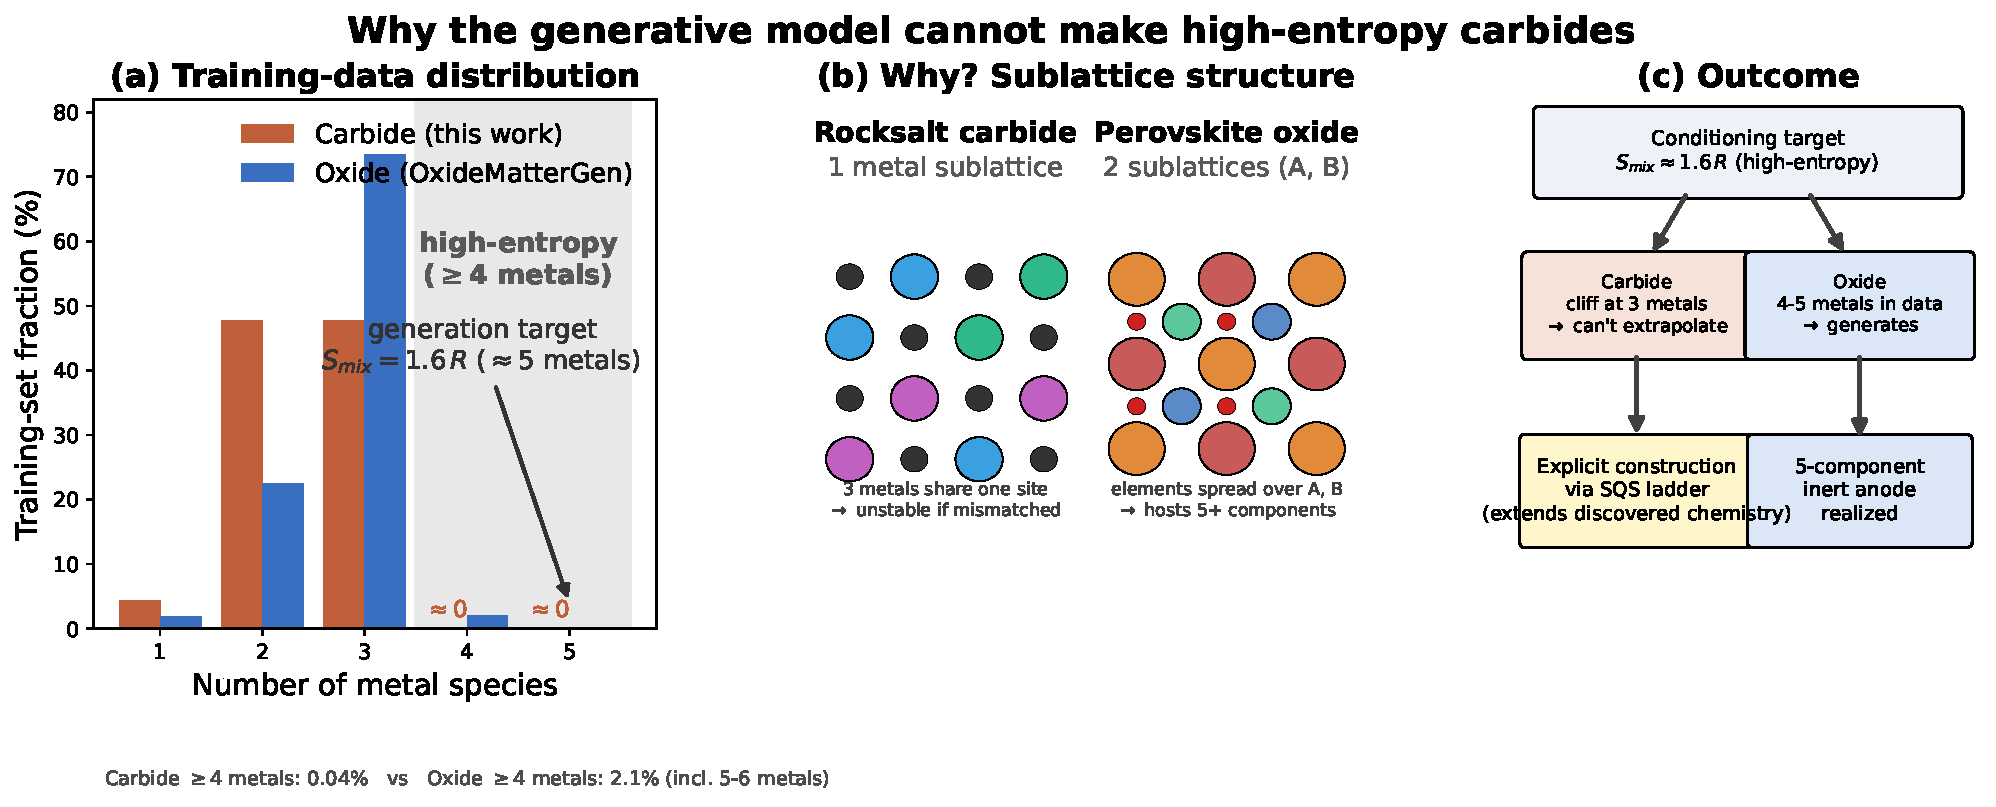
\includegraphics[width=\textwidth]{fig_gen_entropy_limit_en.pdf}
\caption{Why the generative model cannot make high-entropy carbides, and the role of the SQS ladder. (a) Training-set
metal-species-count distribution (measured): the carbides (orange) form a cliff at three metals ($\ge\!4$ metals
$0.04\%$), whereas the oxides (blue, OxideMatterGen) do contain 4--6 metals ($2.1\%$); the conditioning target
$S_{\mathrm{mix}}\!=\!1.6\,R$ is an extrapolation outside the carbide distribution. (b) Root cause: rocksalt carbides
have one metal sublattice (multiple metals compete for one site $\rightarrow$ unstable), whereas perovskite oxides
have two sublattices, A and B (elements accommodated dispersively $\rightarrow$ 5+ components stable). (c) Consequence:
for carbides, generative extrapolation fails $\rightarrow$ explicit construction via the SQS ladder; for oxides, five
components are realized by generation.}
\label{fig:genlimit}
\end{figure}

\section{Multi-Carbon Products and the Multi-Site Tandem Hypothesis}
\label{sec:tandem}
The computational design of this work targeted only CO$_2\!\to\!$CO (two electrons) and HER suppression, yet the
\textsuperscript{1}H NMR of the preliminary electrolysis showed \emph{ethanol} production (Chapter~\ref{ch:experiment};
quantification in progress). Ethanol is a 12-electron, multi-carbon (C\textsubscript{2+}) product that requires
\emph{C--C coupling}, so this is an observation beyond the design goal and requires honest interpretation.

\paragraph{Tension from the single-site view.} At first glance this seems to conflict with the design: the optimized
active site has $\dGCO\!\approx\!0$ (weak binding / release), which by a \emph{single-site} criterion is actually
unfavorable to C--C coupling --- because CO leaves the surface before coupling can occur. That is, the very site we
optimized is a CO \emph{source}, not a coupling site.

\paragraph{Multi-site tandem hypothesis.} This tension is resolved by the essence of the \emph{high-entropy} surface
--- site diversity. The screening ranked each composition by its \emph{optimal} site ($\dGCO\!\approx\!0$), but an
equimolar multi-metal rocksalt surface has a broad $\dGCO$ distribution, and sites that bind CO more strongly also
exist. These strong-binding sites retain CO and let it couple with an adjacent CO to proceed to C\textsubscript{2+},
while the weak-binding sites handle the CO$_2\!\to\!$CO supply. Thus \emph{a single material can act as a tandem
catalyst possessing both CO-production sites and C--C coupling sites}, and the observed ethanol is interpreted as this
emergent multi-site effect. Furthermore, H repulsion (A2, $\dGH>0$) is favorable not only to CO but to \emph{all}
CO\textsubscript{2}RR products --- by suppressing both current loss to HER and $*$H poisoning, it also contributes to
C\textsubscript{2+} selectivity.

\paragraph{Branching verdict: which downstream route is favored (computed).} To partially test this hypothesis, we
computed with UMA the first intermediate of the three fates of $*$CO --- CO release, C1 hydrogenation ($*$CHO), and
C2 coupling ($*$OCCO) --- on the (100) surface of all three candidates (adding $*$CHO/$*$OCCO to the pipeline).
The C--C-coupled $*$OCCO \emph{dissociates} into two CO at most sites, but a physically coupled site
(C--C$\approx$1.5~\AA) survives on all three candidates and its adsorption free energy is \emph{negative}
($\Delta G_{*\mathrm{OCCO}}=-0.56\!\sim\!-1.17$~eV at the coupled site), showing that \textbf{the surface stabilizes
CO--CO coupling}. In contrast, C1 hydrogenation ($*$CHO) is generally \emph{endergonic} ($\sim\!+0.8$~eV). Thus the
calculation indicates that the \textbf{C2 (ethanol) route is favored over C1 (methanol/methane)}, in qualitative
agreement with the experimental observation of ethanol (indicated conceptually in Fig.~\ref{fig:cheher}a).

\paragraph{Limitations and future work.} The branching verdict above is a \emph{falsifiable} partial check, but with
several caveats: (i) only the \emph{first} $*$OCCO coupling intermediate was computed --- the \emph{full} ethanol
pathway (subsequent proton--electron transfers) and the coupling \emph{transition states / barriers} are not computed,
and since most sites dissociate (coupling survives only at specific sites), C--C coupling is a UMA-level (out-of-training-distribution)
\emph{qualitative} signal that requires DFT verification (the $*$OCCO/$*$CHO zero-point corrections are also approximate); (ii) since ethanol
arises from the \emph{site distribution} rather than the optimal site, it is not directly linked to the activity
ranking; (iii) the ethanol-versus-CO partitioning (Faradaic efficiency) is unquantified. Future work is to compute
from first principles the CO--CO coupling energetics across the site distribution and to \emph{add a coupling
descriptor as a conditioning property} so as to actively design C\textsubscript{2+} selectivity. In short, this thesis
designed and validated the \emph{necessary condition} of CO production and HER suppression, and ethanol is an
encouraging experimental result shown by the high-entropy surface on top of that, indicating an extension pathway
toward C\textsubscript{2+}.

\section{Limitations and Honest Caveats}
Several caveats must be stated. (i) The light rare earths (La, Ce, Pr, Y) are economically ``inexpensive'' by the
chosen descriptor, but rare-earth carbides are unusual CO\textsubscript{2}RR catalysts, oxophilic, and may be
sensitive to air/moisture. Experimental robustness is an open problem that the planned stability tests address
directly. (ii) The MLIP surface screening was calibrated to offset baseline error, but it evaluates rare-earth
carbide surfaces that lie mostly outside the learned distribution. In particular, the strongly bound *COOH energy must
be read qualitatively, and the activity ranking relies on the more robust $\dGCO$ descriptor. (iii) The composition
surrogate used in Stages A--B is a literature-based estimate for coarse filtering, not a quantitative prediction.
(iv) DFT treats the rare-earth $4f$ electrons as a fixed trivalent core. This is appropriate for these metallic
carbides, but properties sensitive to the $f$-states require a $4f$-valence or DFT$+U$ treatment. (v) The current DFT
verifies \emph{bulk} stability and metallicity. Explicit disordered \emph{surface} free energies in DFT (on the SQS
supercell of Stage A$'$) are the natural next computational step beyond the MLIP-level surface screening reported here.
These limitations motivate rather than weaken the experimental campaign of Chapter~\ref{ch:experiment}, and experiment
is the arbiter of the predictions.

\section{Outlook}
Beyond confirming the Ti-based candidates of Campaign B, the contrast between the two campaigns demonstrated the
value of \emph{placing the constraint in the generative stage}: when the generator was re-aimed at low VEC in
Campaign B, the model itself yielded H-repelling candidates, suggesting that discovery can come from conditioning
rather than a post-processing screen. The pipeline supports an active-learning loop in which experimental and
higher-level DFT data recalibrate the composition surrogate and the MLIP to refine successive generations. The same
conditional generator can be re-aimed at CO\textsubscript{2}-to-formate or multi-carbon products by changing the
conditioning descriptors.

% =====================================================================
\chapter{Conclusion}
\label{ch:conclusion}

This thesis internalized the four design axioms of a superior CO\textsubscript{2}RR carbide catalyst (activity,
selectivity, manufacturability, economics) in a property-conditioned diffusion model and, \emph{driving a single
pipeline with two constraint sets}, validated them through a funnel of machine-learning potentials and first-principles
DFT. \emph{Campaign A} (the activity-first baseline) derived six platinum-group-free high-entropy carbides from 1024
generated structures and characterized them by surface free energy, $d$-band, convex hull, and same-facet surface
Pourbaix (at the operating potential the steady state is the reaction intermediate $*$COOH, not oxidation). This
candidate group, however, is eliminated at the \emph{manufacturability gate} --- the rare earths dissolve during the
essential leaching step of metallothermic-reduction--\emph{acid-leaching} synthesis and are thus unmanufacturable.
This is not a failure but a controlled contrast, showing that \emph{unconstrained activity search converges to an
unmanufacturable chemistry} and demonstrating the need to promote manufacturability to a generative constraint.

\emph{Campaign B} imposes all four axioms: it restricts the search space to acid-leaching-stable group-4/5/6
transition metals (excluding, along with rare earths and platinum-group metals, the known CO$_2$RR metals
Cu/Ag/Au/Zn as well, to secure the discovery contribution of the generative model), conditions on UMA-computed
surface labels, and explicitly addresses HER competition --- because strong H adsorption is a \emph{poisoning} that
covers the CO$_2$ sites --- applying a \emph{dual active-site} criterion that simultaneously demands CO evolution
($|\dGCO|<0.3$) and \emph{H repulsion} ($\dGH>0$) on the same facet. Rare earths are excluded for manufacturing and
are also \emph{unnecessary} for the active-site design, because the dual behavior is a valence-electron-concentration
(VEC) effect of the transition metals (the two rationales are independent). As a result, \textbf{three Ti-based
three-metal rocksalt carbides (hec3-MoTiZr/CrTiV/CrTiZr, (100)) passed the DFT dual objective}, confirming that H
poisoning is the dominant failure mode and that low VEC is the physical lever that jointly tunes H repulsion and CO
evolution. Full ionic relaxation of the representative candidate hec3-MoTiZr \emph{confirms the selectivity}
($\dGH\!=\!+0.57$~eV, actually strengthened; $\dGCO\!=\!+0.18$~eV) while \emph{correcting the limiting potential to
$U_L\!=\!-0.40$~V}, showing that the single-point calculation had underestimated the $*$COOH barrier. Finally,
re-aiming the generator at low VEC caused \emph{the generative model itself} to yield H-repelling, CO-evolving
winners, demonstrating that discovery can come from conditional generation rather than a post-processing screen.

To test these predictions, an experimental validation program consisting of synthesis, electrochemical
CO\textsubscript{2}RR, online gas analysis, \textsuperscript{1}H NMR, and in-situ FT-IR was designed
(Chapter~\ref{ch:experiment}). The broader contribution is to show, reusably, that economics, \emph{synthesizability},
and \emph{HER selectivity} can all be taken as \emph{generative} design goals in catalyst discovery, that synthetic
reality (acid leaching) defines the elemental palette, and that physics (hydrogen poisoning) defines the conditioning
lever (VEC).

% =====================================================================
\begin{thebibliography}{99}
\setlength{\itemsep}{2pt}

\bibitem{zeni2025} C.~Zeni, R.~Pinsler, D.~Z\"ugner, A.~Fowler, M.~Horton, X.~Fu, Z.~Wang,
A.~Shysheya, J.~Crabb\'e, S.~Shysheya, \emph{et al.},
``A generative model for inorganic materials design,''
\emph{Nature} \textbf{639}, 624--632 (2025). doi:10.1038/s41586-025-08628-5.

\bibitem{uma2025} B.~M.~Wood, M.~Dzamba, X.~Fu, M.~Gao, M.~Shuaibi, L.~Barroso-Luque,
K.~Abdelmaqsoud, V.~Gharakhanyan, J.~R.~Kitchin, \emph{et al.},
``UMA: A Family of Universal Models for Atoms,'' arXiv:2506.23971 (2025).

\bibitem{chanussot2021} L.~Chanussot, A.~Das, S.~Goyal, T.~Lavril, M.~Shuaibi, M.~Riviere,
K.~Tran, J.~Heras-Domingo, C.~Ho, W.~Hu, \emph{et al.},
``Open Catalyst 2020 (OC20) Dataset and Community Challenges,''
\emph{ACS Catal.} \textbf{11}, 6059--6072 (2021). doi:10.1021/acscatal.0c04525.

\bibitem{giannozzi2009} P.~Giannozzi, S.~Baroni, N.~Bonini, M.~Calandra, R.~Car, C.~Cavazzoni,
D.~Ceresoli, G.~L.~Chiarotti, M.~Cococcioni, I.~Dabo, \emph{et al.},
``QUANTUM ESPRESSO: a modular and open-source software project for quantum simulations of
materials,'' \emph{J. Phys.: Condens. Matter} \textbf{21}, 395502 (2009).
doi:10.1088/0953-8984/21/39/395502.

\bibitem{prandini2018} G.~Prandini, A.~Marrazzo, I.~E.~Castelli, N.~Mounet, N.~Marzari,
``Precision and efficiency in solid-state pseudopotential calculations,''
\emph{npj Comput. Mater.} \textbf{4}, 72 (2018). doi:10.1038/s41524-018-0127-2.

\bibitem{pbe1996} J.~P.~Perdew, K.~Burke, M.~Ernzerhof,
``Generalized Gradient Approximation Made Simple,''
\emph{Phys. Rev. Lett.} \textbf{77}, 3865--3868 (1996). doi:10.1103/PhysRevLett.77.3865.

\bibitem{norskov2004} J.~K.~N\o{}rskov, J.~Rossmeisl, A.~Logadottir, L.~Lindqvist,
J.~R.~Kitchin, T.~Bligaard, H.~J\'onsson,
``Origin of the Overpotential for Oxygen Reduction at a Fuel-Cell Cathode,''
\emph{J. Phys. Chem. B} \textbf{108}, 17886--17892 (2004). doi:10.1021/jp047349j.

\bibitem{nitopi2019} S.~Nitopi, E.~Bertheussen, S.~B.~Scott, X.~Liu, A.~K.~Engstfeld, S.~Horch,
B.~Seger, I.~E.~L.~Stephens, K.~Chan, C.~Hahn, J.~K.~N\o{}rskov, T.~F.~Jaramillo, I.~Chorkendorff,
``Progress and Perspectives of Electrochemical CO\textsubscript{2} Reduction on Copper in Aqueous
Electrolyte,'' \emph{Chem. Rev.} \textbf{119}, 7610--7672 (2019).
doi:10.1021/acs.chemrev.8b00705.

\bibitem{hori2008} Y.~Hori, ``Electrochemical CO\textsubscript{2} Reduction on Metal Electrodes,''
in \emph{Modern Aspects of Electrochemistry}, vol.~42, eds.\ C.~G.~Vayenas \emph{et al.},
Springer, New York, pp.~89--189 (2008). doi:10.1007/978-0-387-49489-0\_3.

\bibitem{batchelor2019} T.~A.~A.~Batchelor, J.~K.~Pedersen, S.~H.~Winther, I.~E.~Castelli,
K.~W.~Jacobsen, J.~Rossmeisl,
``High-Entropy Alloys as a Discovery Platform for Electrocatalysis,''
\emph{Joule} \textbf{3}, 834--845 (2019). doi:10.1016/j.joule.2018.12.015.

\bibitem{nellaiappan2020} S.~Nellaiappan, N.~K.~Katiyar, R.~Kumar, A.~Parui, K.~D.~Malviya,
K.~G.~Pradeep, A.~K.~Singh, S.~Sharma, C.~S.~Tiwary, K.~Biswas,
``High-Entropy Alloys as Catalysts for the CO\textsubscript{2} and CO Reduction Reactions:
Experimental Realization,'' \emph{ACS Catal.} \textbf{10}, 3658--3663 (2020).
doi:10.1021/acscatal.9b04302.

\bibitem{levy1973} R.~B.~Levy, M.~Boudart,
``Platinum-Like Behavior of Tungsten Carbide in Surface Catalysis,''
\emph{Science} \textbf{181}, 547--549 (1973). doi:10.1126/science.181.4099.547.

\bibitem{porosoff2014} M.~D.~Porosoff, X.~Yang, J.~A.~Boscoboinik, J.~G.~Chen,
``Molybdenum Carbide as Alternative Catalysts to Precious Metals for Highly Selective Reduction of
CO\textsubscript{2} to CO,'' \emph{Angew. Chem. Int. Ed.} \textbf{53}, 6705--6709 (2014).
doi:10.1002/anie.201404109.

\bibitem{sarker2018} P.~Sarker, T.~Harrington, C.~Toher, C.~Oses, M.~Samiee, J.-P.~Maria,
D.~W.~Brenner, K.~S.~Vecchio, S.~Curtarolo,
``High-entropy high-hardness metal carbides discovered by entropy descriptors,''
\emph{Nat. Commun.} \textbf{9}, 4980 (2018). doi:10.1038/s41467-018-07160-7.

\bibitem{zunger1990} A.~Zunger, S.-H.~Wei, L.~G.~Ferreira, J.~E.~Bernard,
``Special quasirandom structures,'' \emph{Phys. Rev. Lett.} \textbf{65}, 353--356 (1990).
doi:10.1103/PhysRevLett.65.353.

\bibitem{pymatgen2013} S.~P.~Ong, W.~D.~Richards, A.~Jain, G.~Hautier, M.~Kocher, S.~Cholia,
D.~Gunter, V.~L.~Chevrier, K.~A.~Persson, G.~Ceder,
``Python Materials Genomics (pymatgen): A robust, open-source python library for materials
analysis,'' \emph{Comput. Mater. Sci.} \textbf{68}, 314--319 (2013).
doi:10.1016/j.commatsci.2012.10.028.

\bibitem{ase2017} A.~Hjorth Larsen, J.~J.~Mortensen, J.~Blomqvist, I.~E.~Castelli, R.~Christensen,
M.~Du\l{}ak, J.~Friis, M.~N.~Groves, B.~Hammer, C.~Hargus, \emph{et al.},
``The atomic simulation environment---a Python library for working with atoms,''
\emph{J. Phys.: Condens. Matter} \textbf{29}, 273002 (2017). doi:10.1088/1361-648X/aa680e.

\end{thebibliography}

\end{document}
